\chapter{MVA Supplementaries}
\label{chap:apdx_mvasupp}

\begin{figure}[htbp]
    \centering
    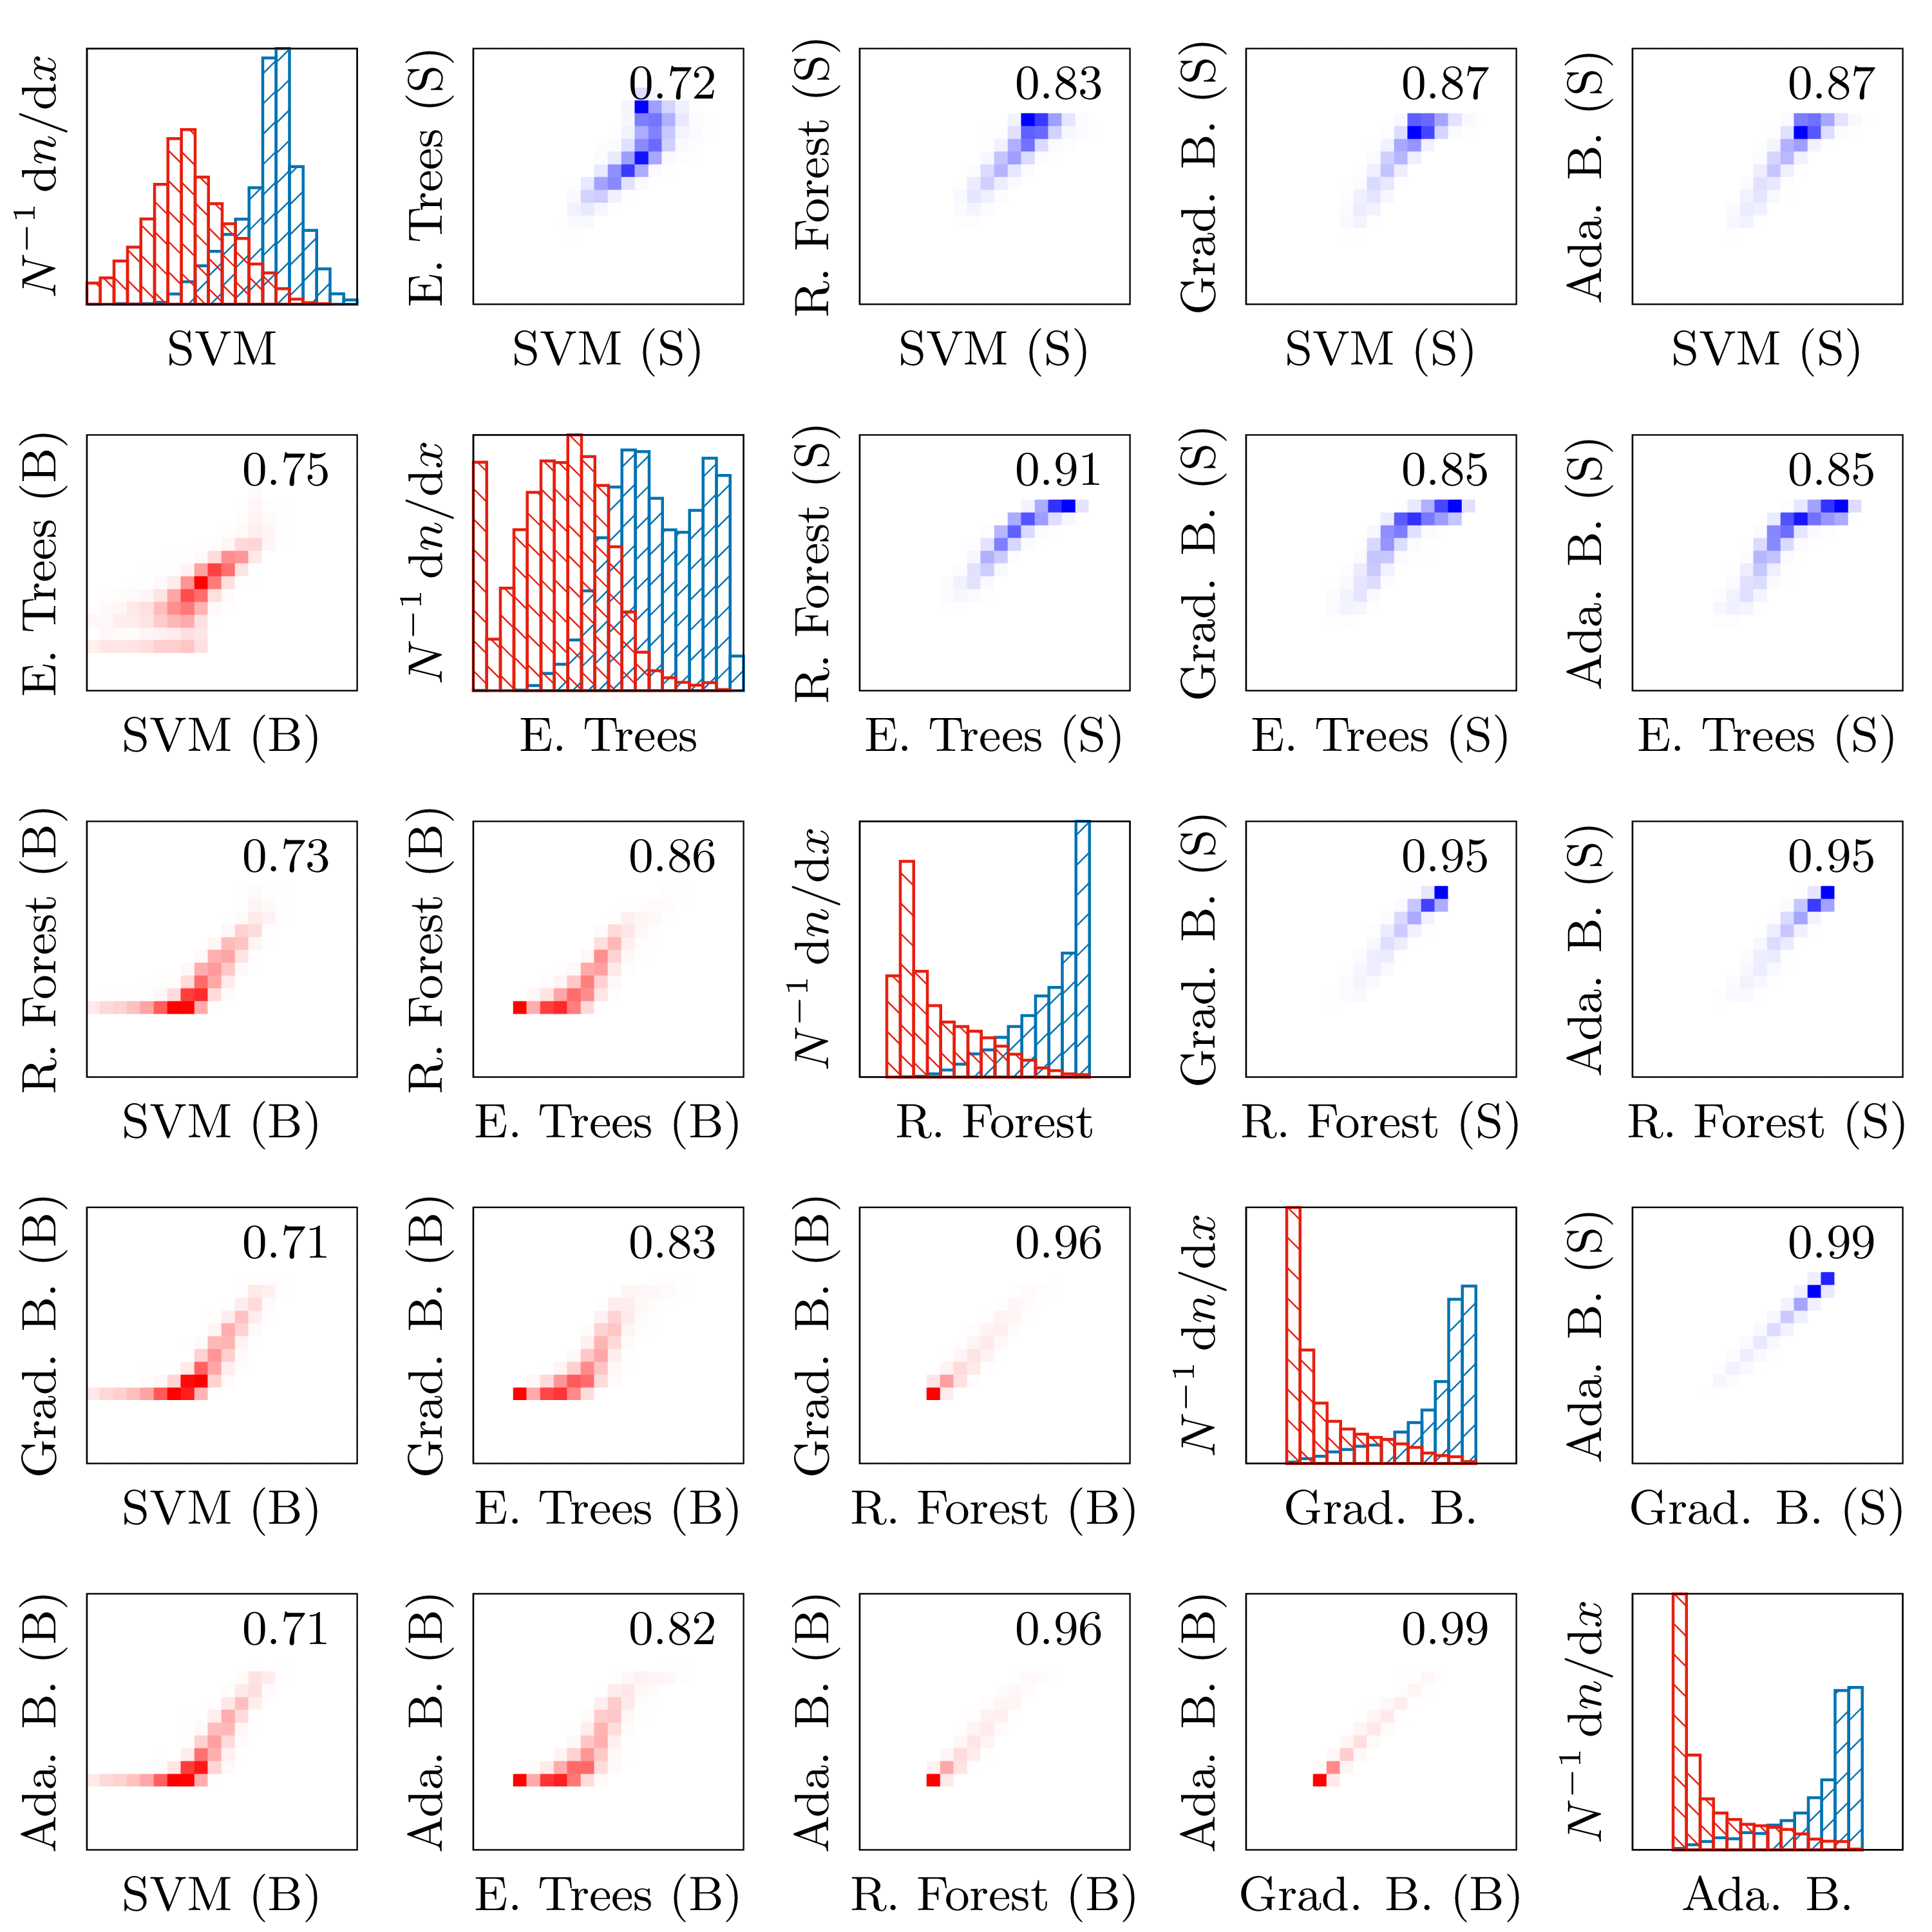
\includegraphics[scale=1.]{mvaLz/stack_features_LL.png}
    \caption{Distributions of the responses and correlations of the tier~1.1 \Lz classifiers for \gls{LL} tracks, separated for signal (S) and background (B). On top of the correlation distributions we show the \gls{pcc} as a measure for the linear correlation.}
    \label{fig:mvaLz_stack_features_LL}
\end{figure}

\begin{figure}[htbp]
    \centering
    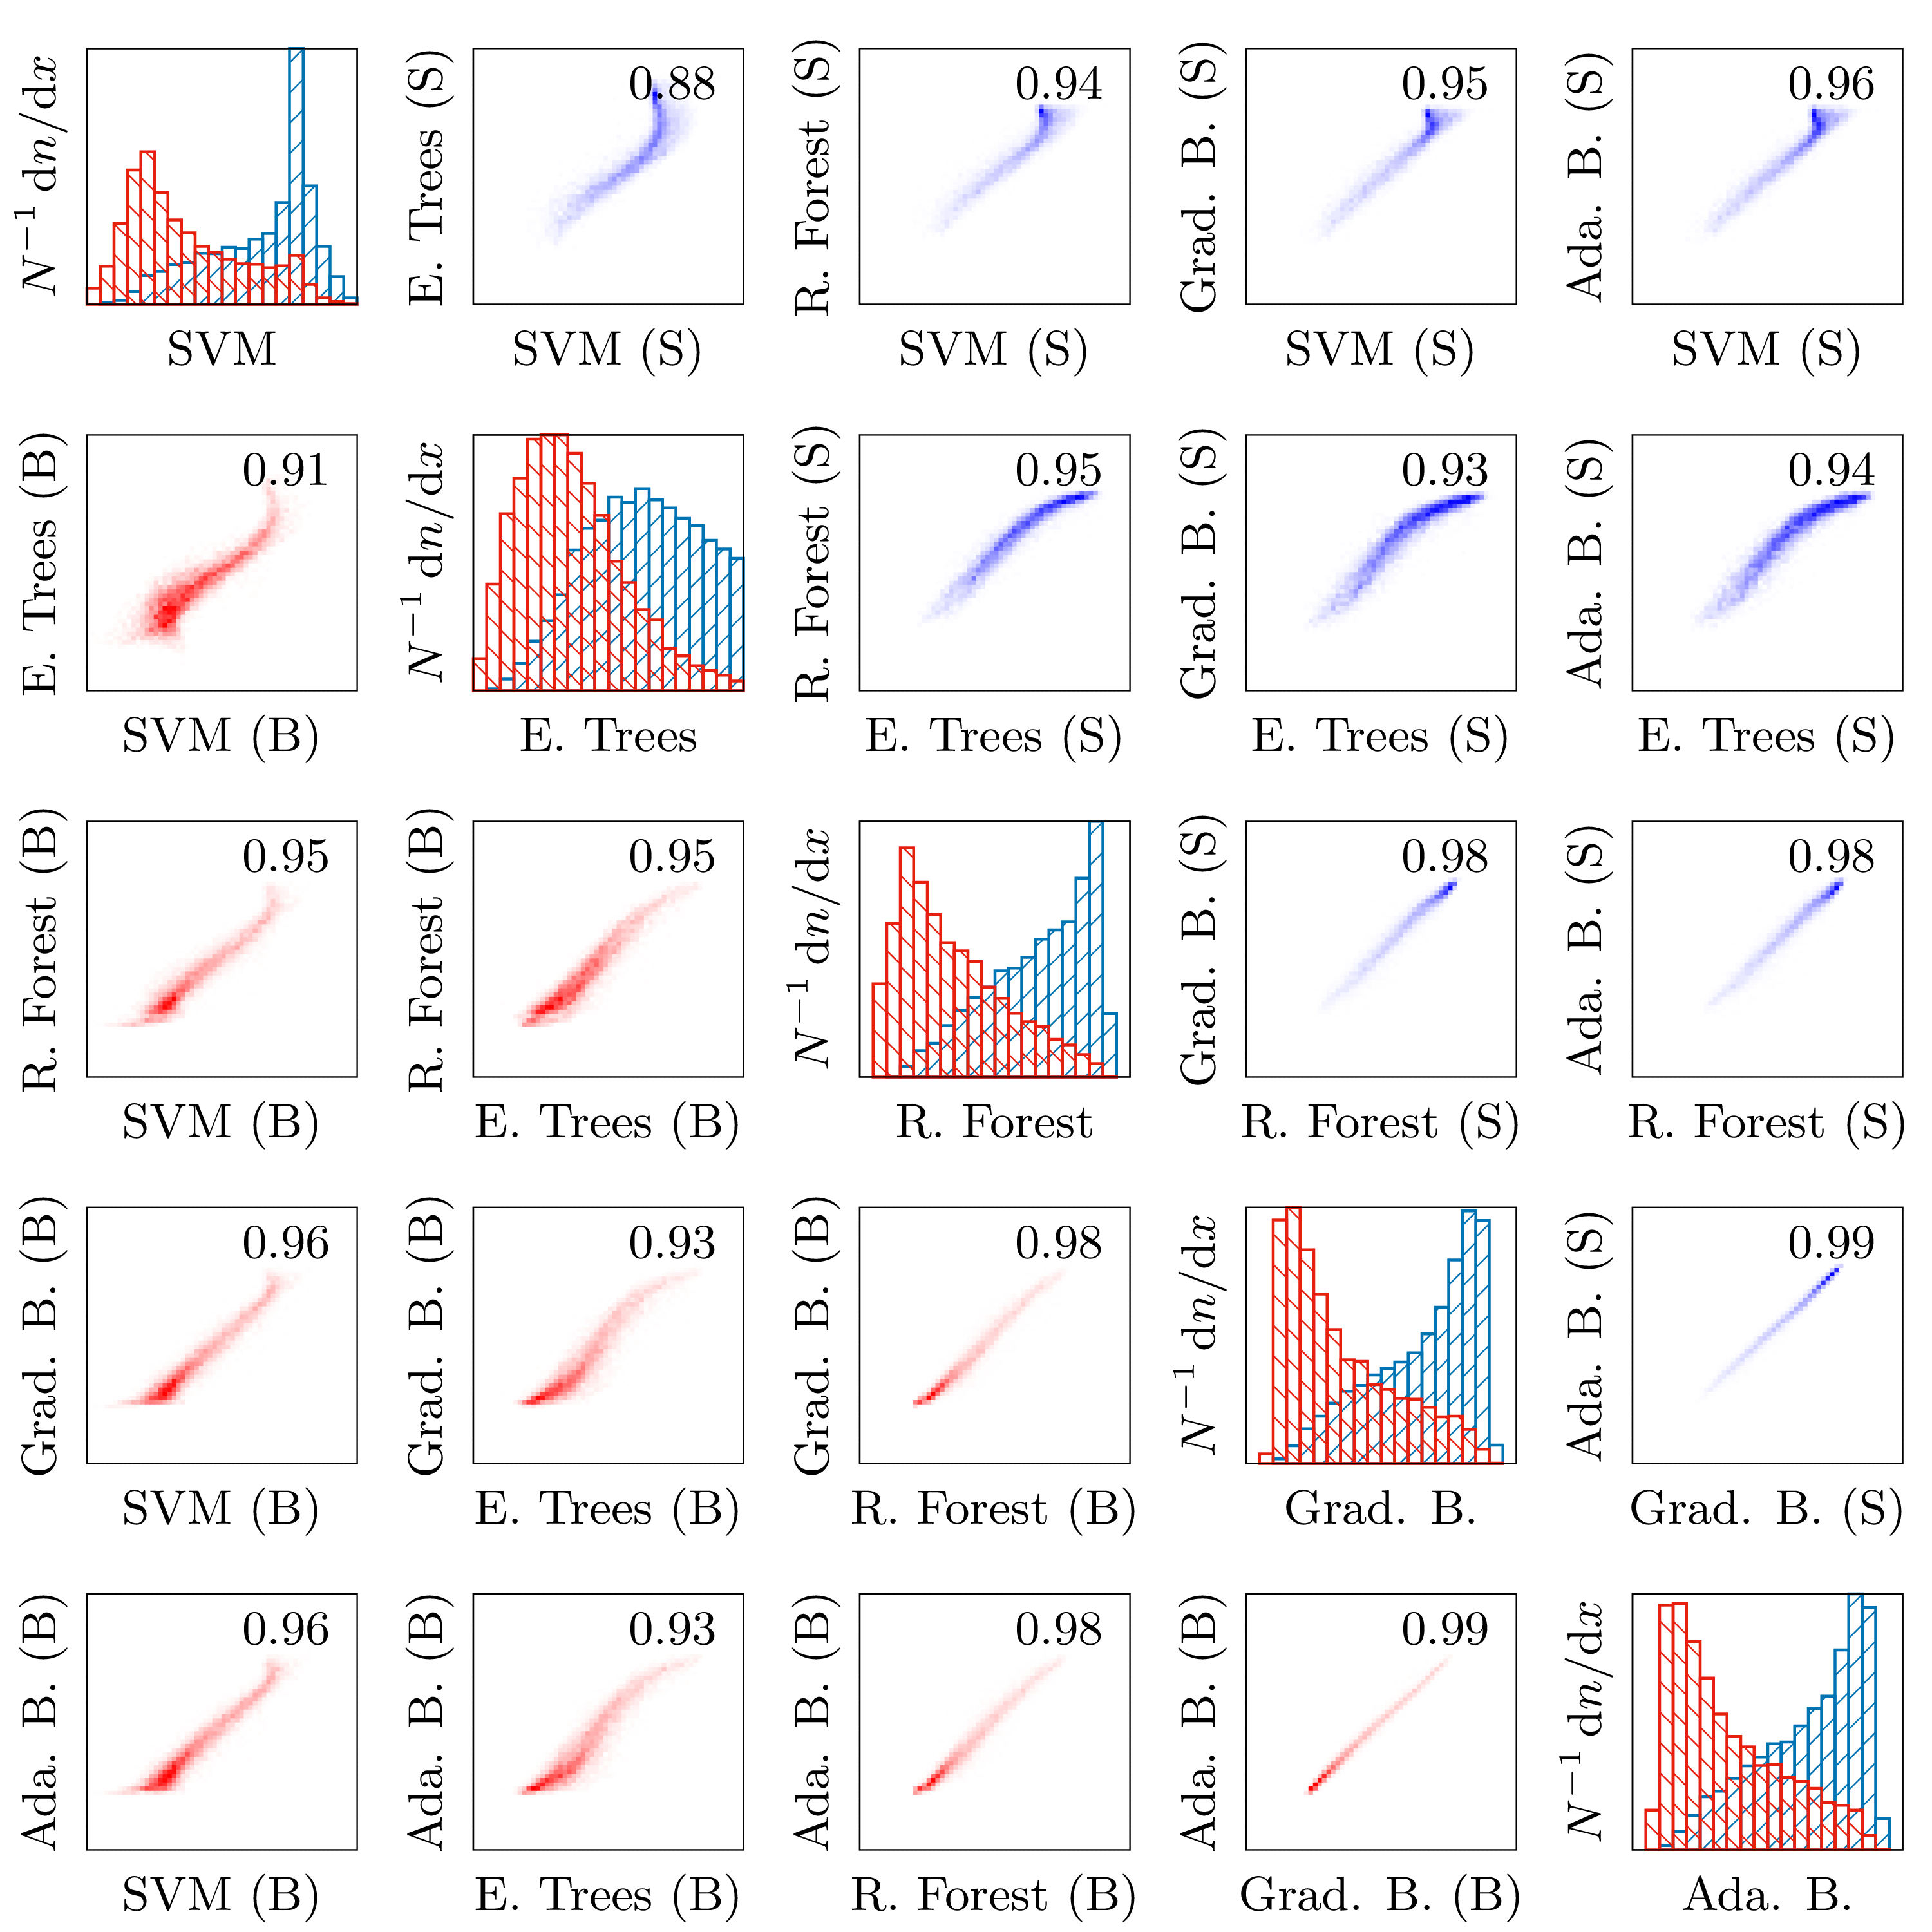
\includegraphics[scale=1.]{mvaLz/stack_features_DD.png}
    \caption{Distributions of the responses and correlations of the tier~1.1 \Lz classifiers for \gls{DD} tracks, separated for signal (S) and background (B). On top of the correlation distributions we show the \gls{pcc} as a measure for the linear correlation.}
    \label{fig:mvaLz_stack_features_DD}
\end{figure}

\begin{figure}[htbp]
    \centering
    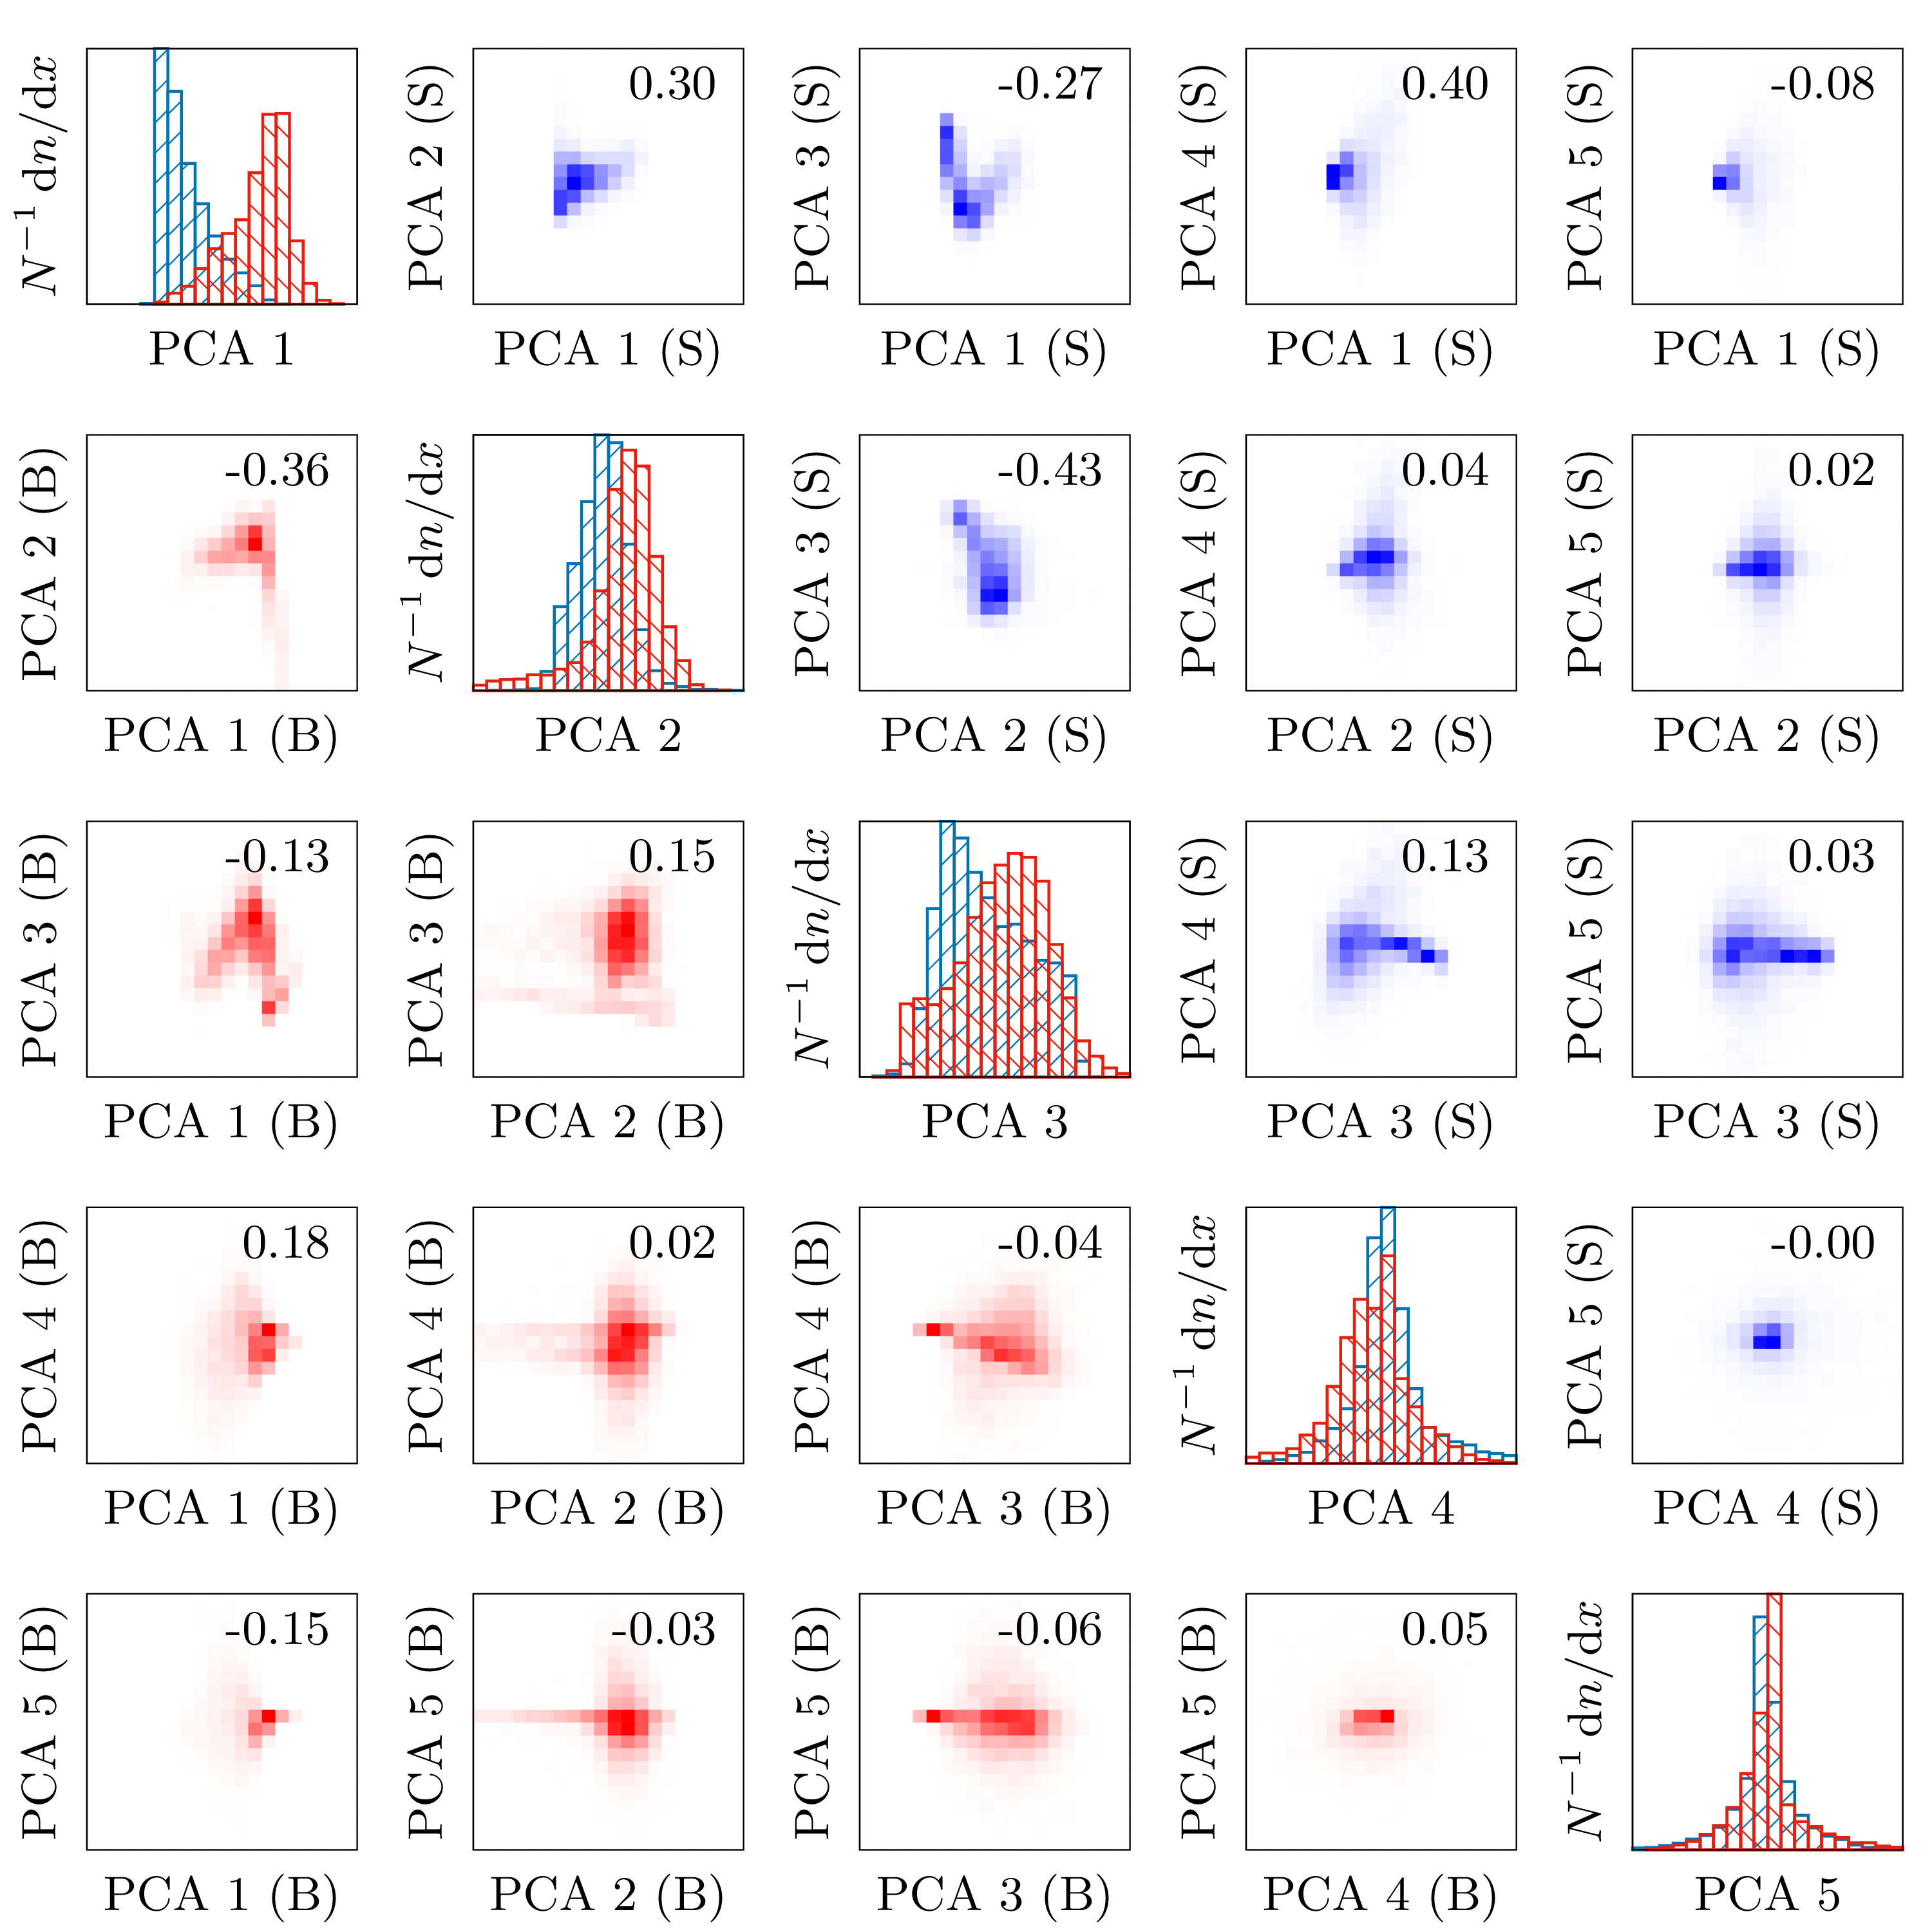
\includegraphics[scale=1.]{mvaLz/stack_pcafeatures_LL.png}
    \caption{Distributions of the responses and correlations of the tier~1.1 \Lz classifiers for \gls{LL} tracks after \gls{pca} transformation, separated for signal (S) and background (B). On top of the correlation distributions we show the \gls{pcc} as a measure for the linear correlation.}
    \label{fig:mvaLz_stack_pcafeatures_LL}
\end{figure}

\begin{figure}[htbp]
    \centering
    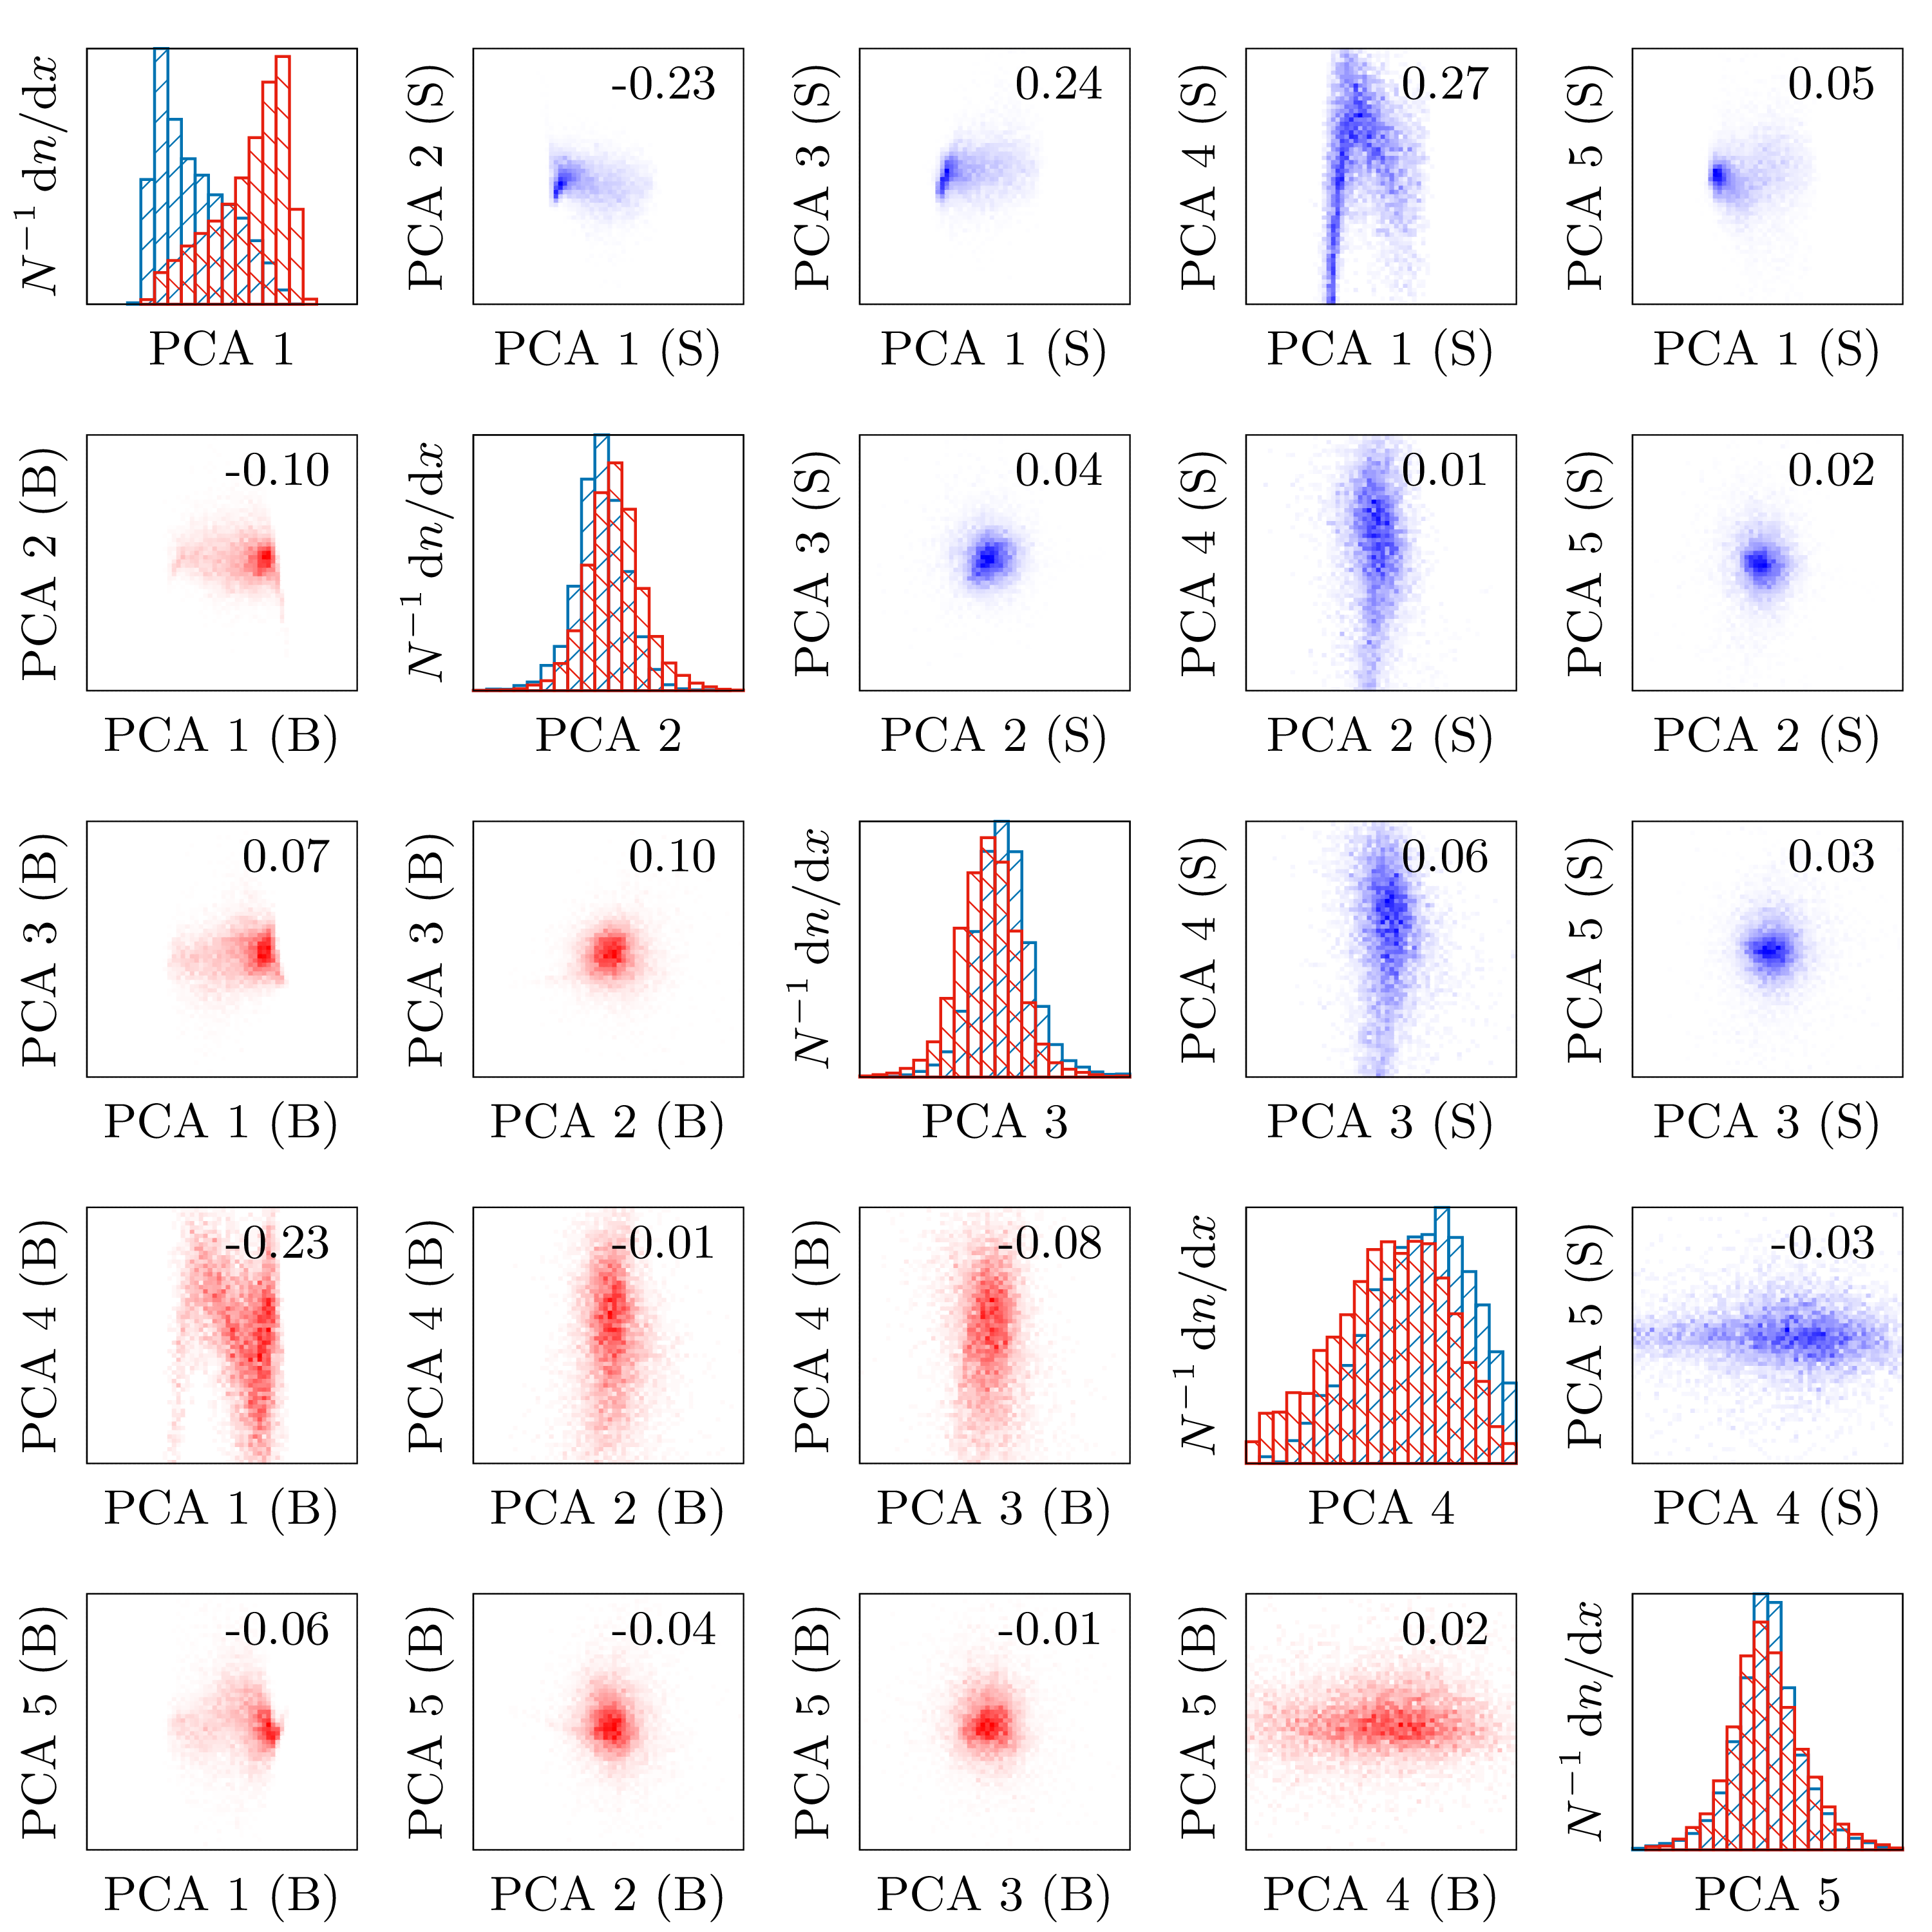
\includegraphics[scale=1.]{mvaLz/stack_pcafeatures_DD.png}
    \caption{Distributions of the responses and correlations of the tier~1.1 \Lz classifiers for \gls{DD} tracks after \gls{pca} transformation, separated for signal (S) and background (B). On top of the correlation distributions we show the \gls{pcc} as a measure for the linear correlation.}
    \label{fig:mvaLz_stack_pcafeatures_DD}
\end{figure}

\begin{figure}[htbp]
    \centering
    \begin{subfigure}[b]{.49\textwidth}
        \centering
        \includegraphics[scale=1.]{mvaLz/roc.png}
        \caption{\Lz classifier}
    \end{subfigure}
    \begin{subfigure}[b]{.49\textwidth}
        \centering
        \includegraphics[scale=1.]{mvaLbDz/roc.png}
        \caption{\Lb-\Dz classifier}
    \end{subfigure}
    \caption{\Gls{roc} curves of the \glspl{svm} used as the \Lz classifier (left) and \Lb-\Dz classifier (right) for \gls{LL} and \gls{DD} tracks.}
    \label{fig:mvaLzLbDz_roc}
\end{figure}

\begin{figure}[htbp]
    \centering
    \begin{subfigure}[b]{.49\textwidth}
        \centering
        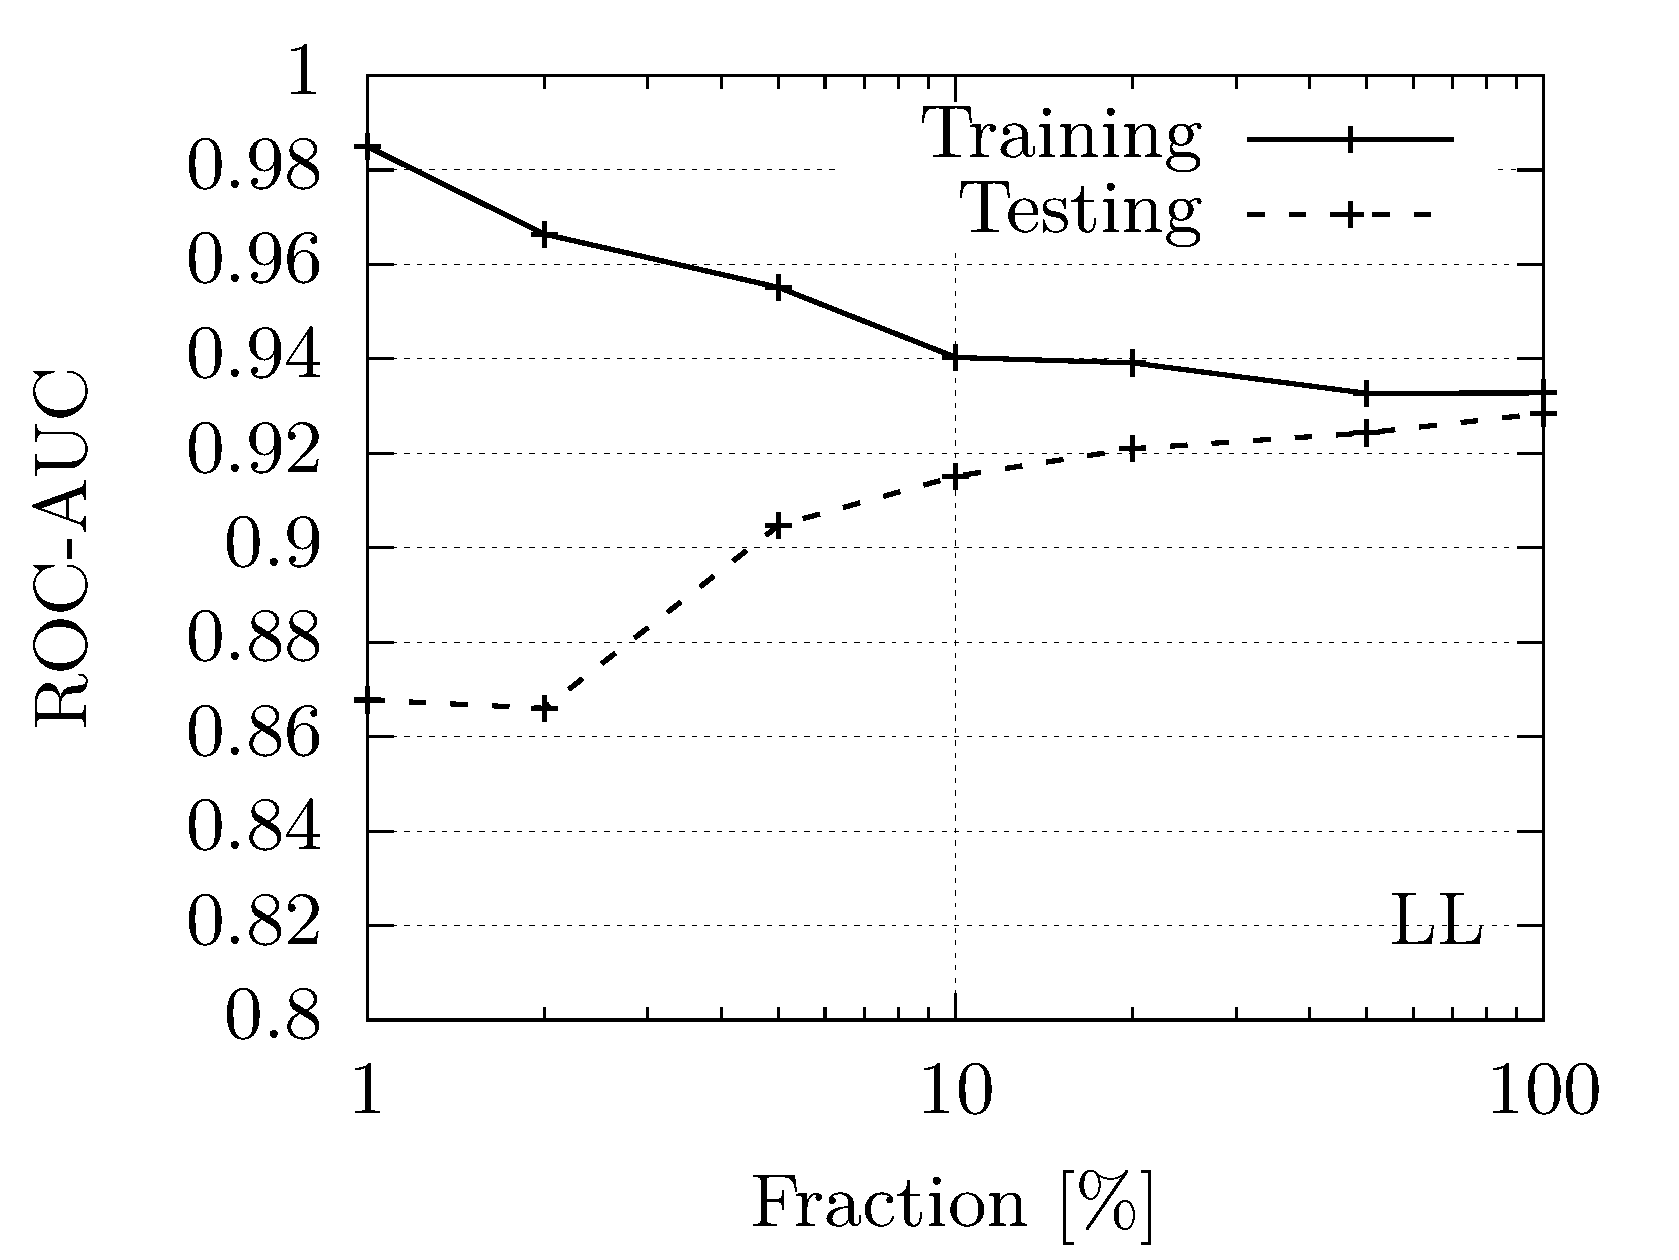
\includegraphics[scale=1.]{mvaLbDz/convergence_LL.png}
    \end{subfigure}
    \begin{subfigure}[b]{.49\textwidth}
        \centering
        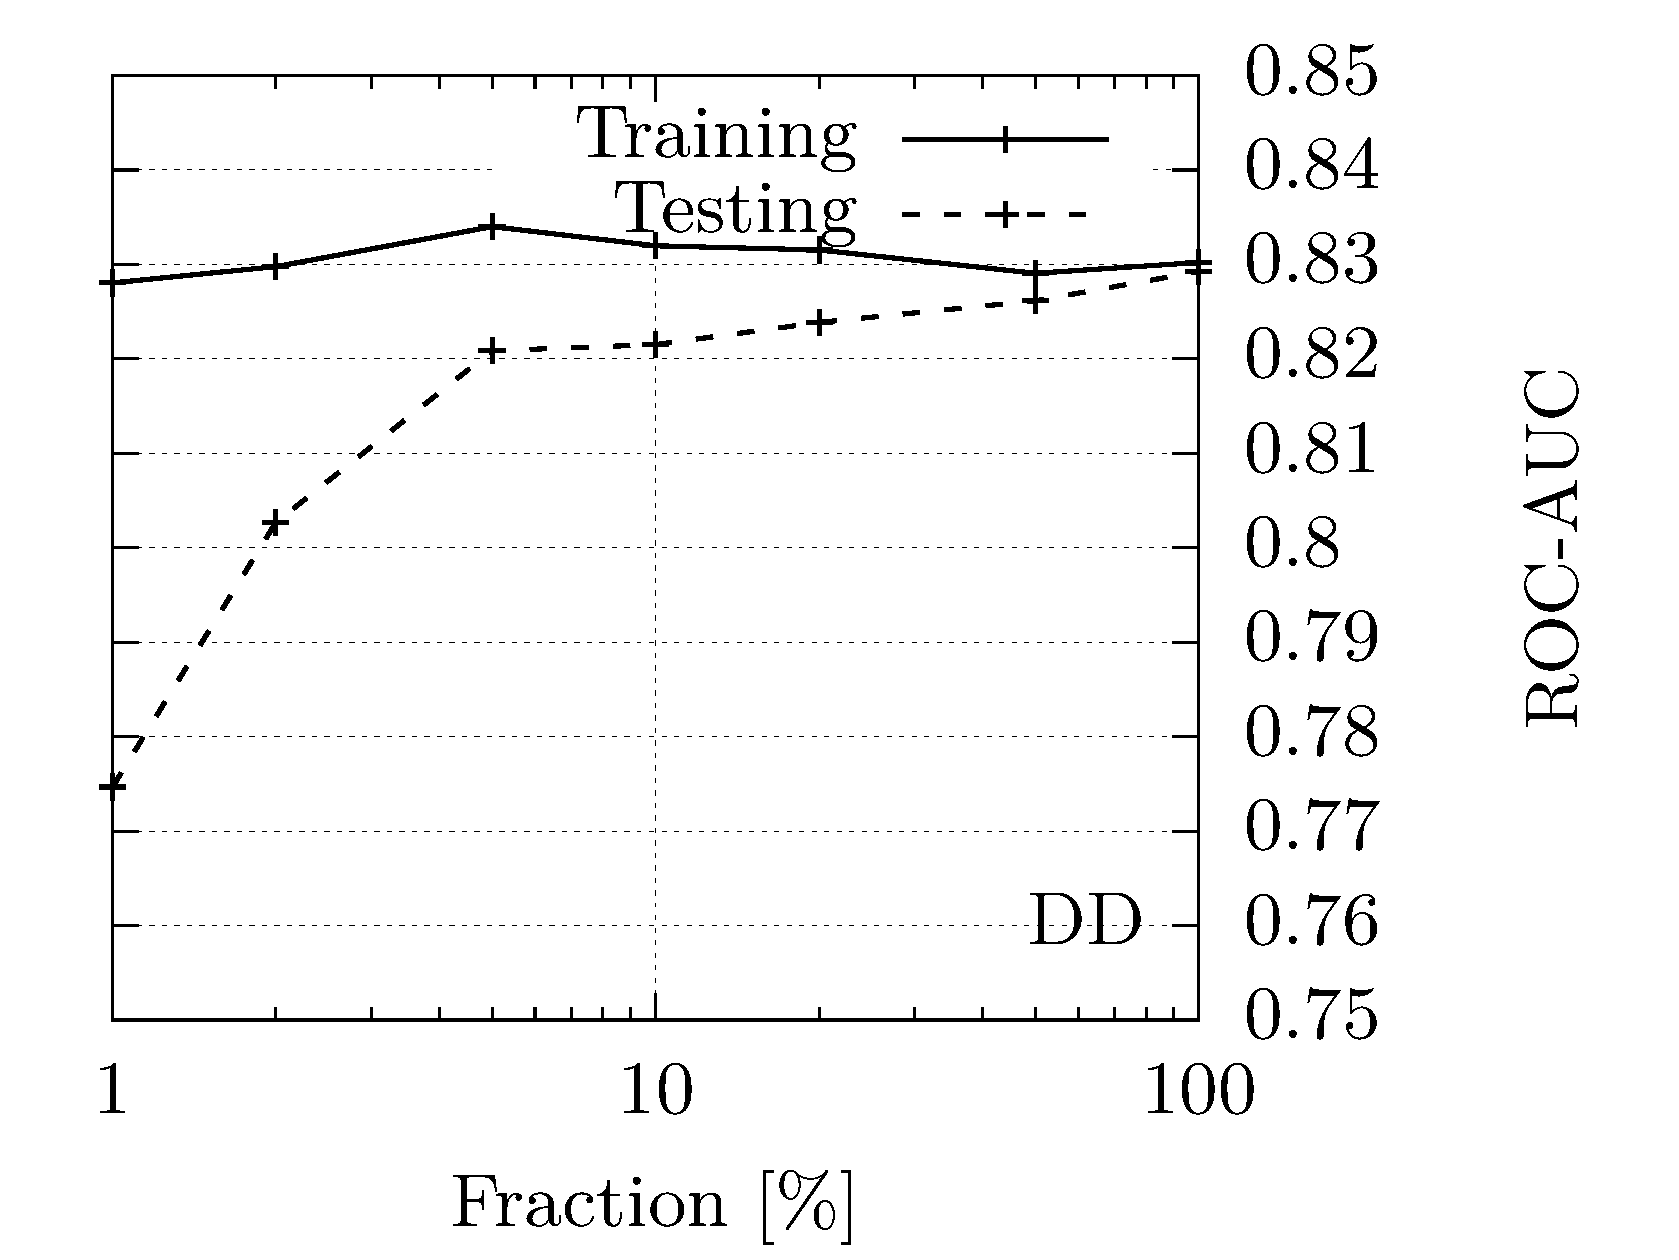
\includegraphics[scale=1.]{mvaLbDz/convergence_DD.png}
    \end{subfigure}
    \caption{Convergence of the \glspl{svm} (\Lb-\Dz classifier) given by the \gls{rocauc} values for different sample sizes where a sample size of $100\,\%$ corresponds to the size of the full trainings set. The \gls{rocauc} is evaluated via a 5-fold cross-validation scheme on the training (solid line) and testing folds (dashed line).}
    \label{fig:mvaLbDz_convergence}
\end{figure}

\begin{figure}[htbp]
    \centering
    \begin{subfigure}[b]{.49\textwidth}
        \centering
        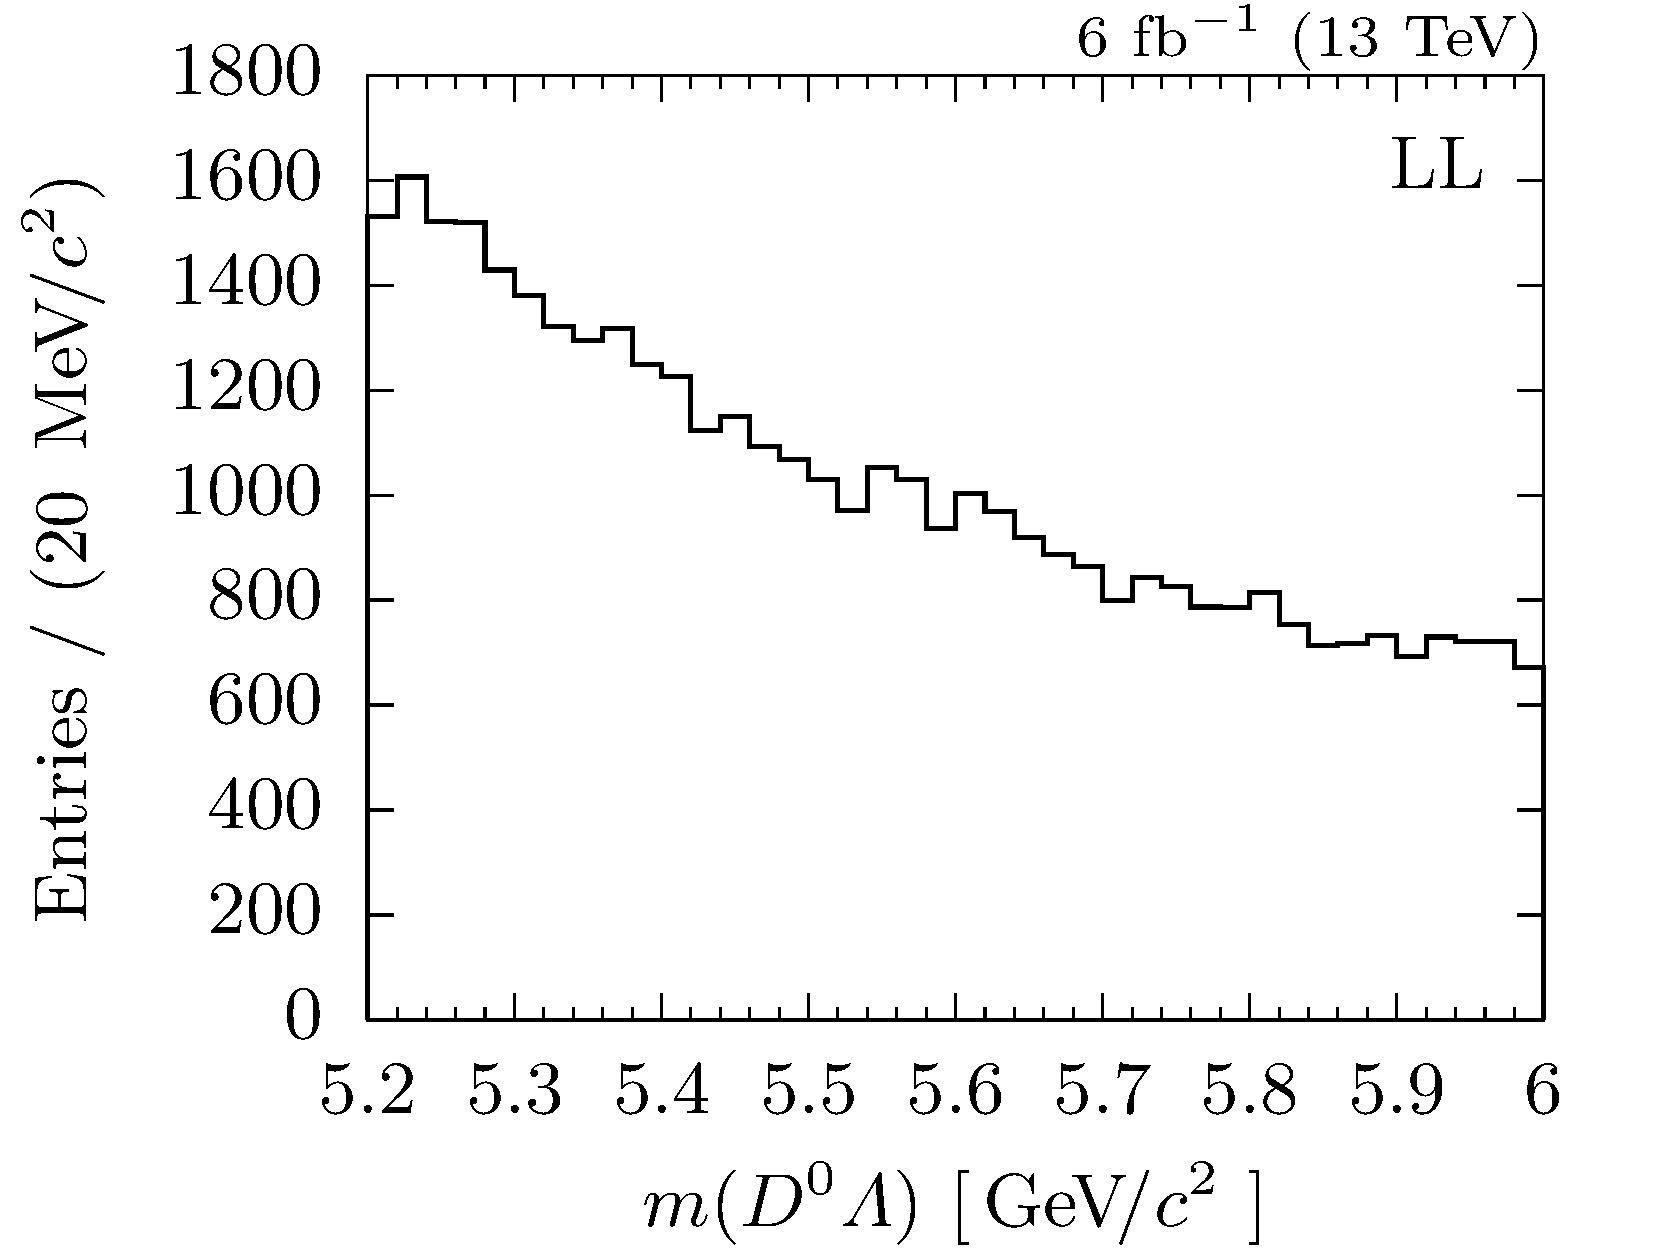
\includegraphics[scale=1.]{mvaLbDz/hDzLzM_LL.png}
    \end{subfigure}
    \begin{subfigure}[b]{.49\textwidth}
        \centering
        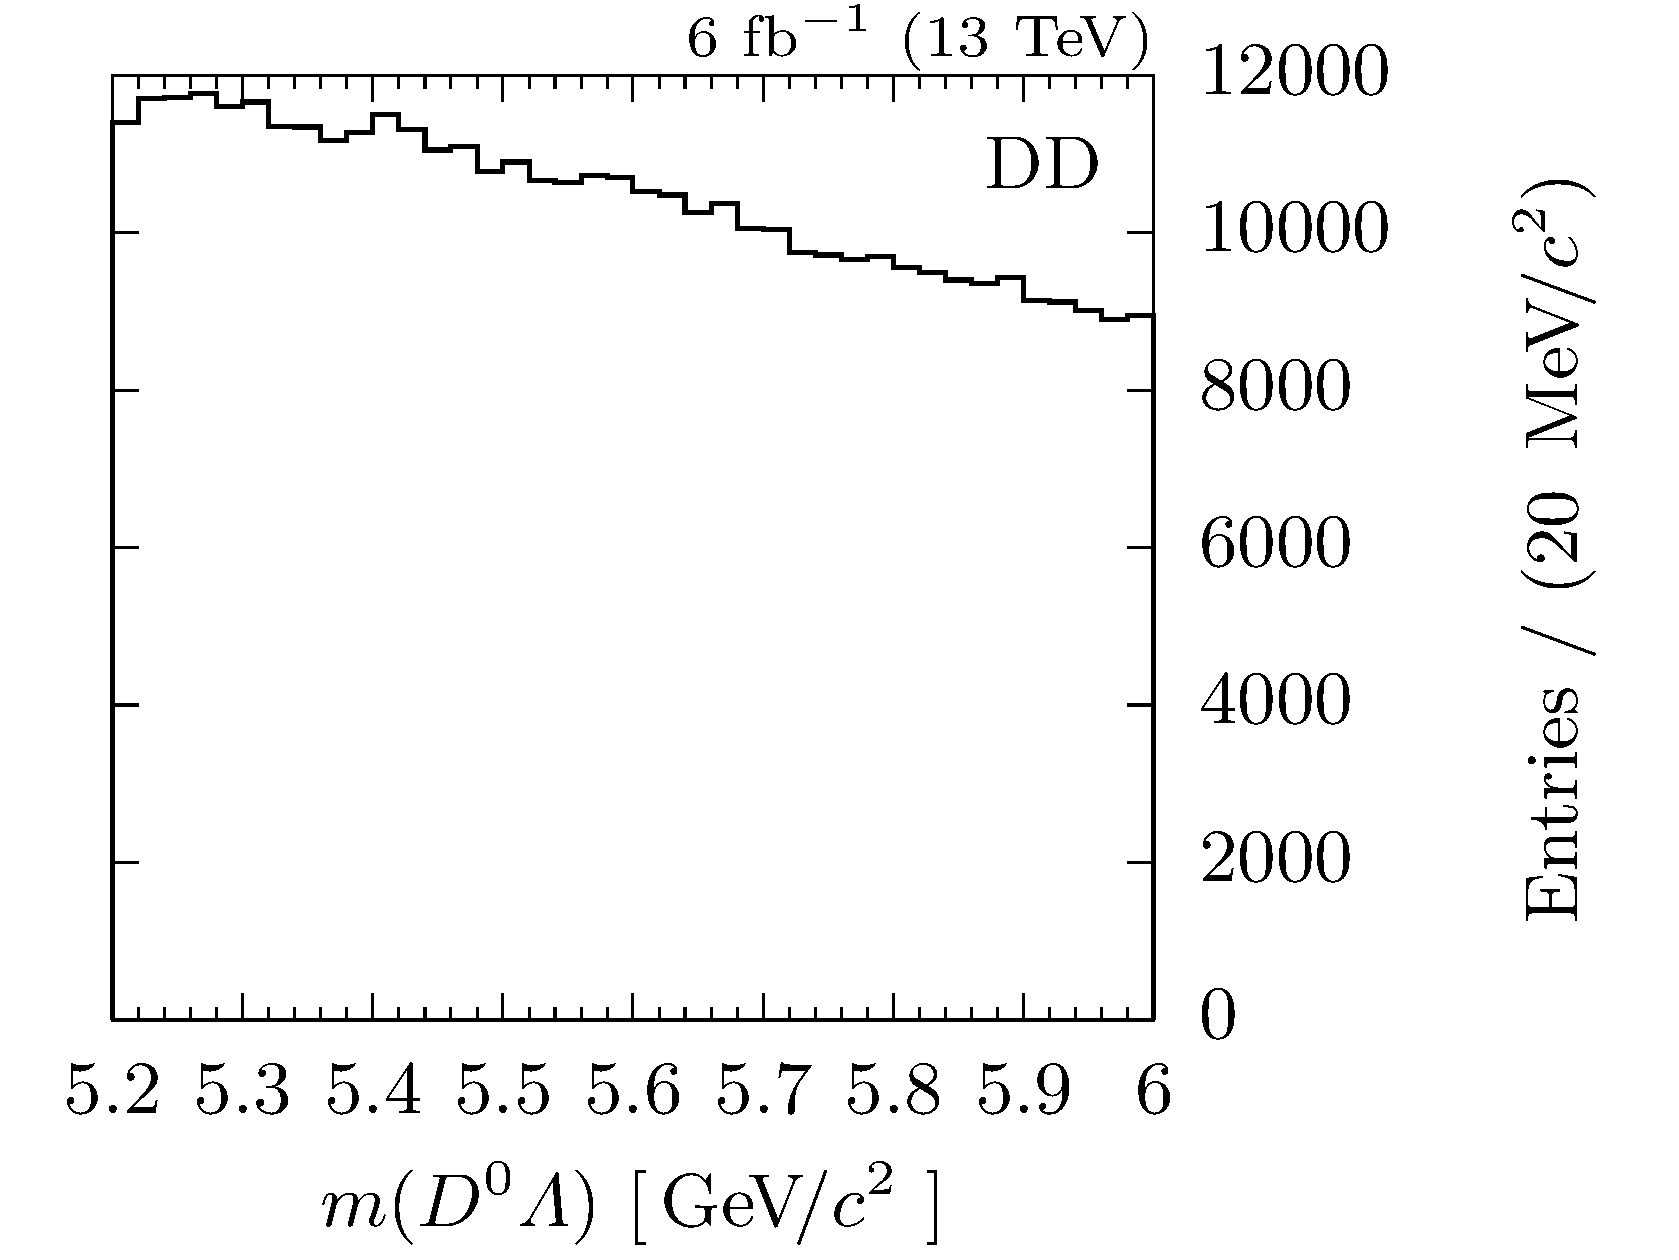
\includegraphics[scale=1.]{mvaLbDz/hDzLzM_DD.png}
    \end{subfigure}
    \caption{Combined invariant mass of \Dz and \Lz candidates after loose selection from recorded data, as used for training the \Lb-\Dz classifier (background class).}
    \label{fig:mvaLbDz_hDzLzM}
\end{figure}

\begin{figure}[htbp]
    \centering
    \begin{subfigure}{.49\textwidth}
        \centering
        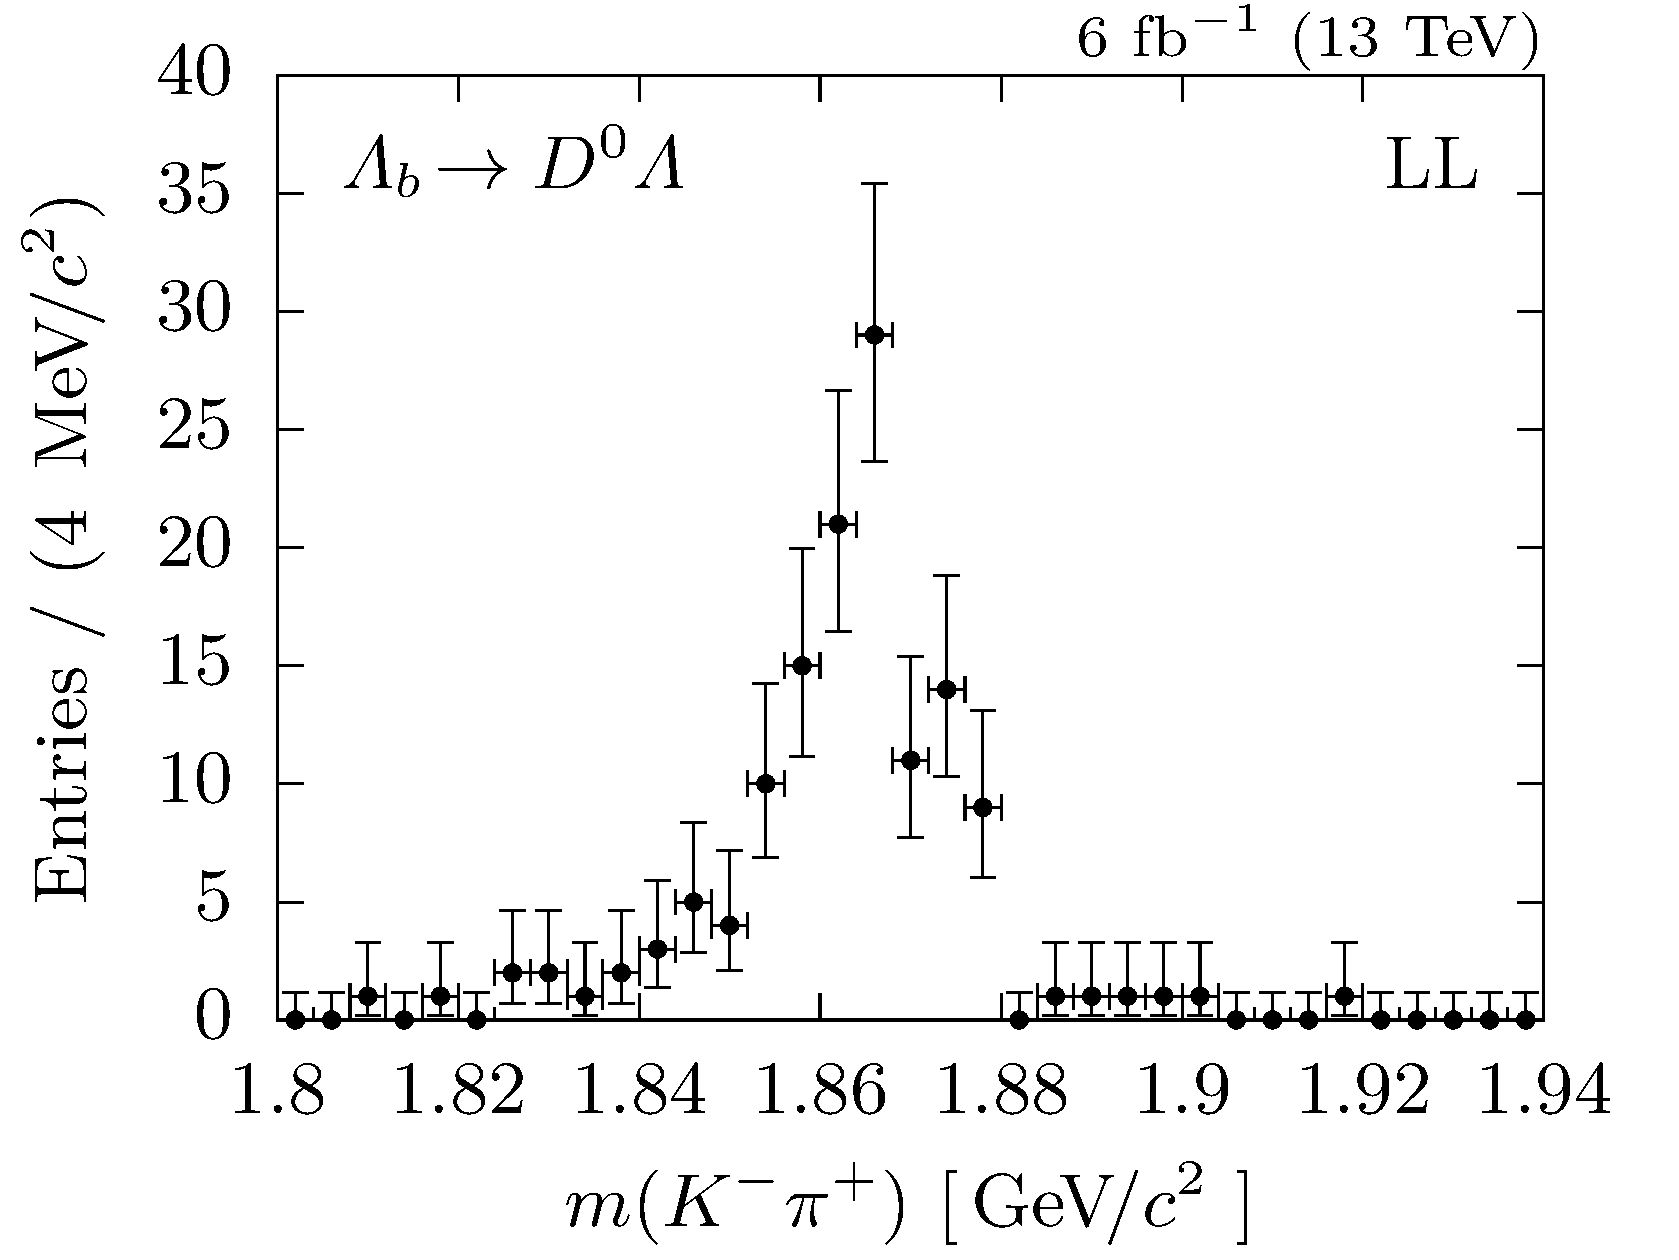
\includegraphics[scale=1.]{mva/hDzM_LL.png}
    \end{subfigure}
    \begin{subfigure}{.49\textwidth}
        \centering
        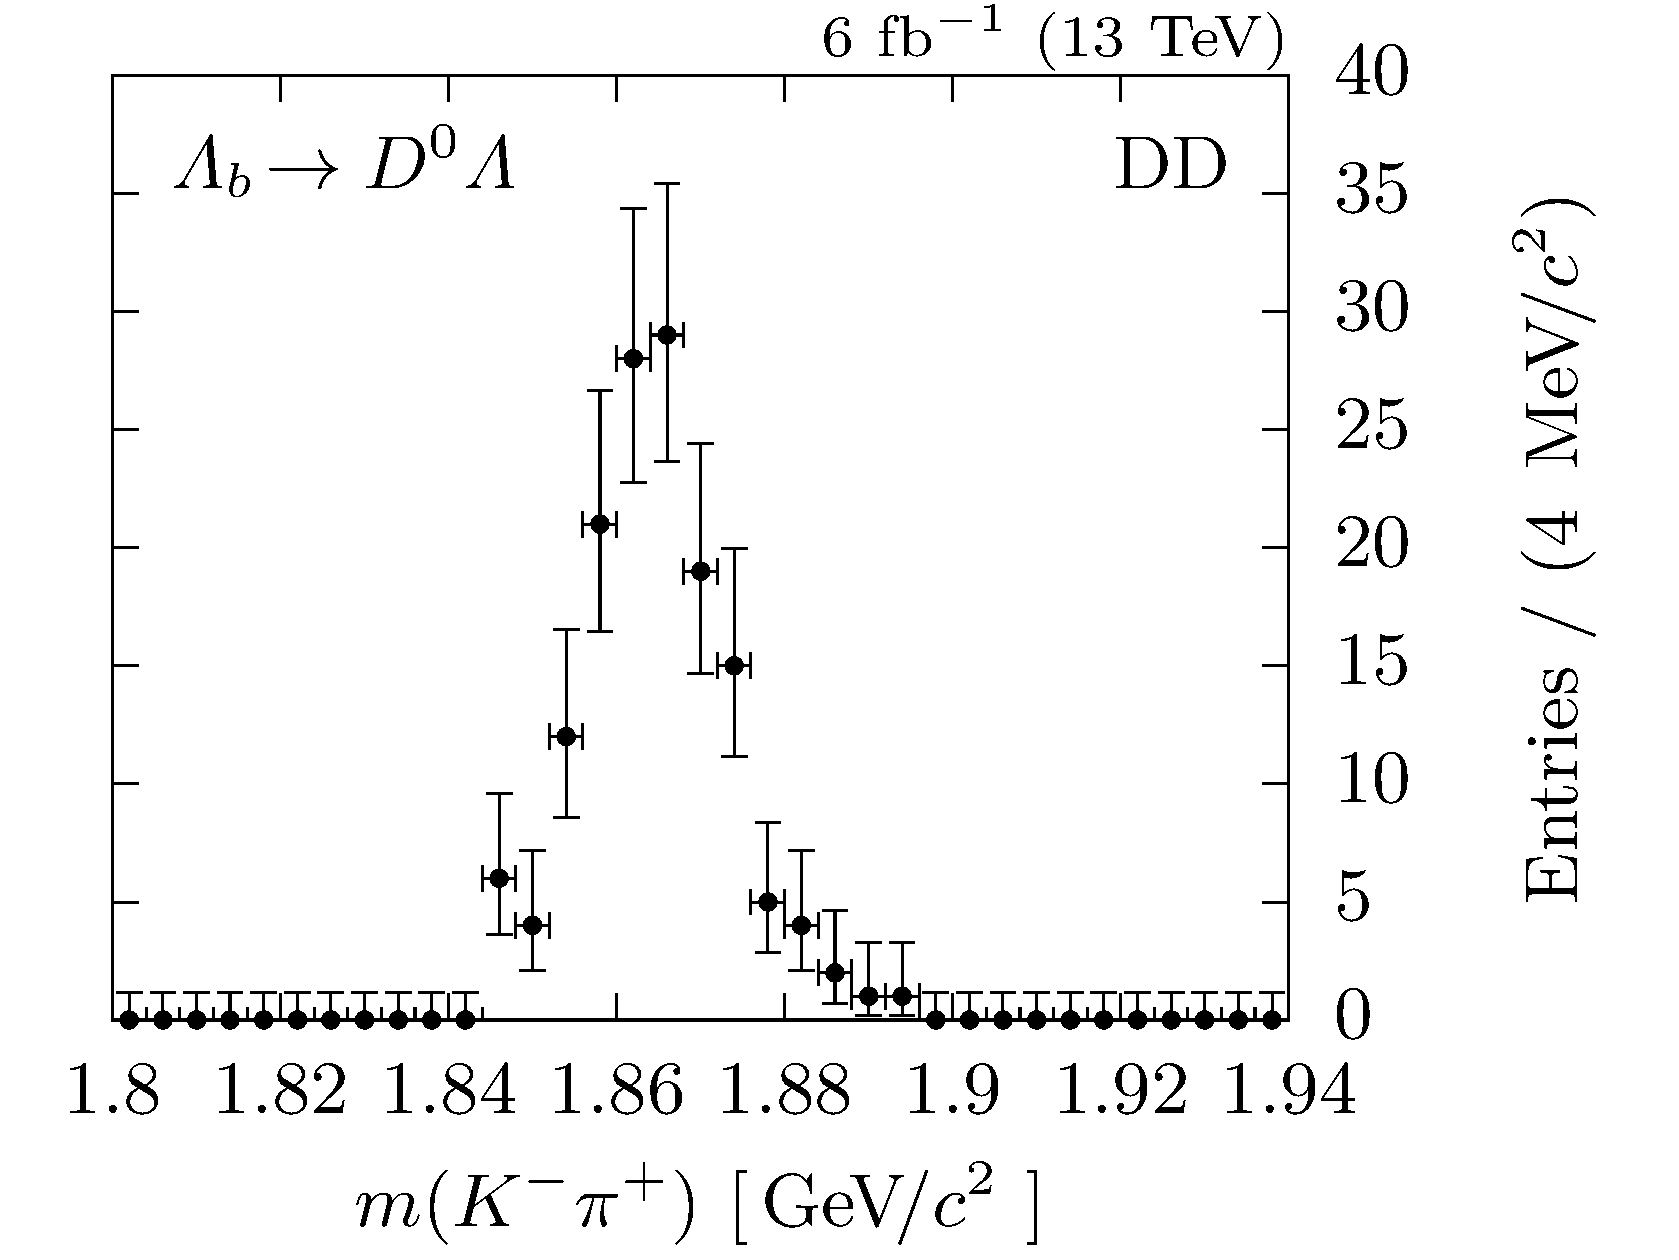
\includegraphics[scale=1.]{mva/hDzM_DD.png}
    \end{subfigure}
    \par\bigskip 
    \begin{subfigure}{.49\textwidth}
        \centering
        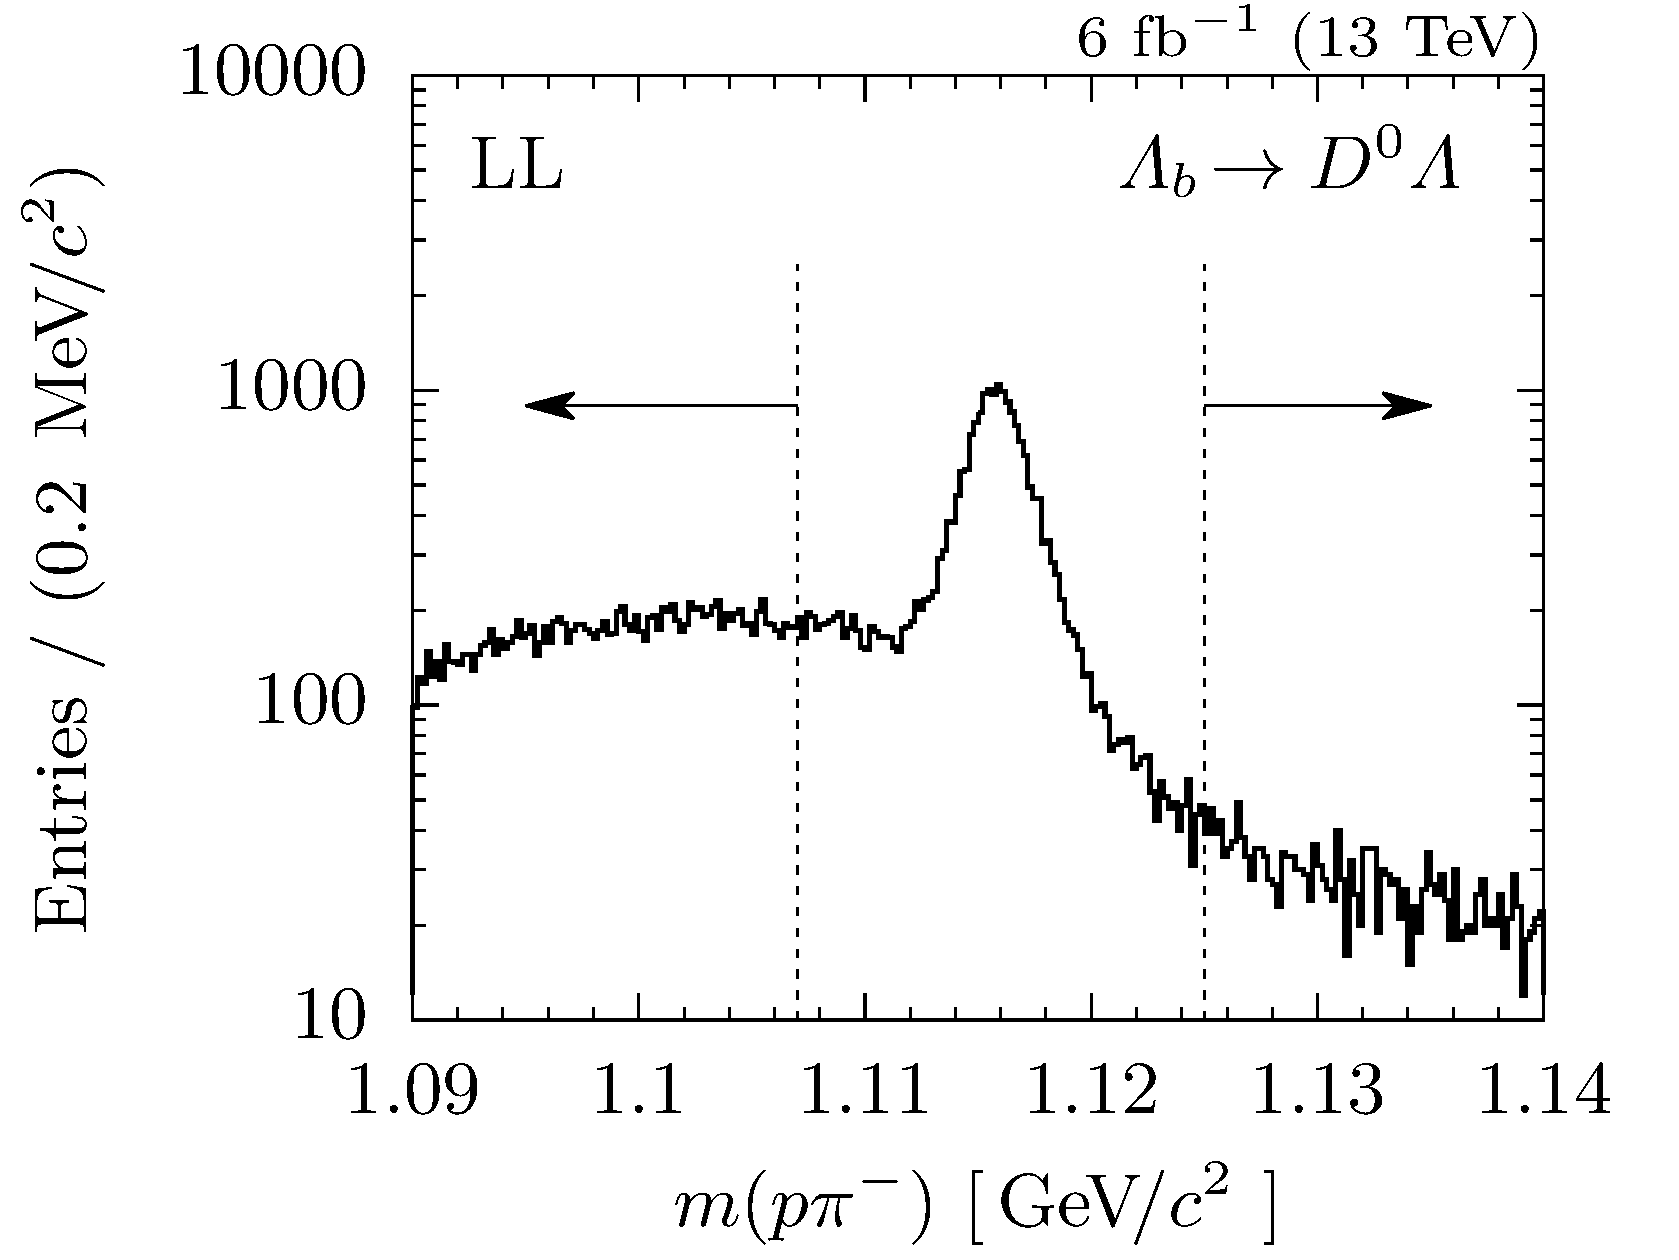
\includegraphics[scale=1.]{mva/hLzM_LL.png}
    \end{subfigure}
    \begin{subfigure}{.49\textwidth}
        \centering
        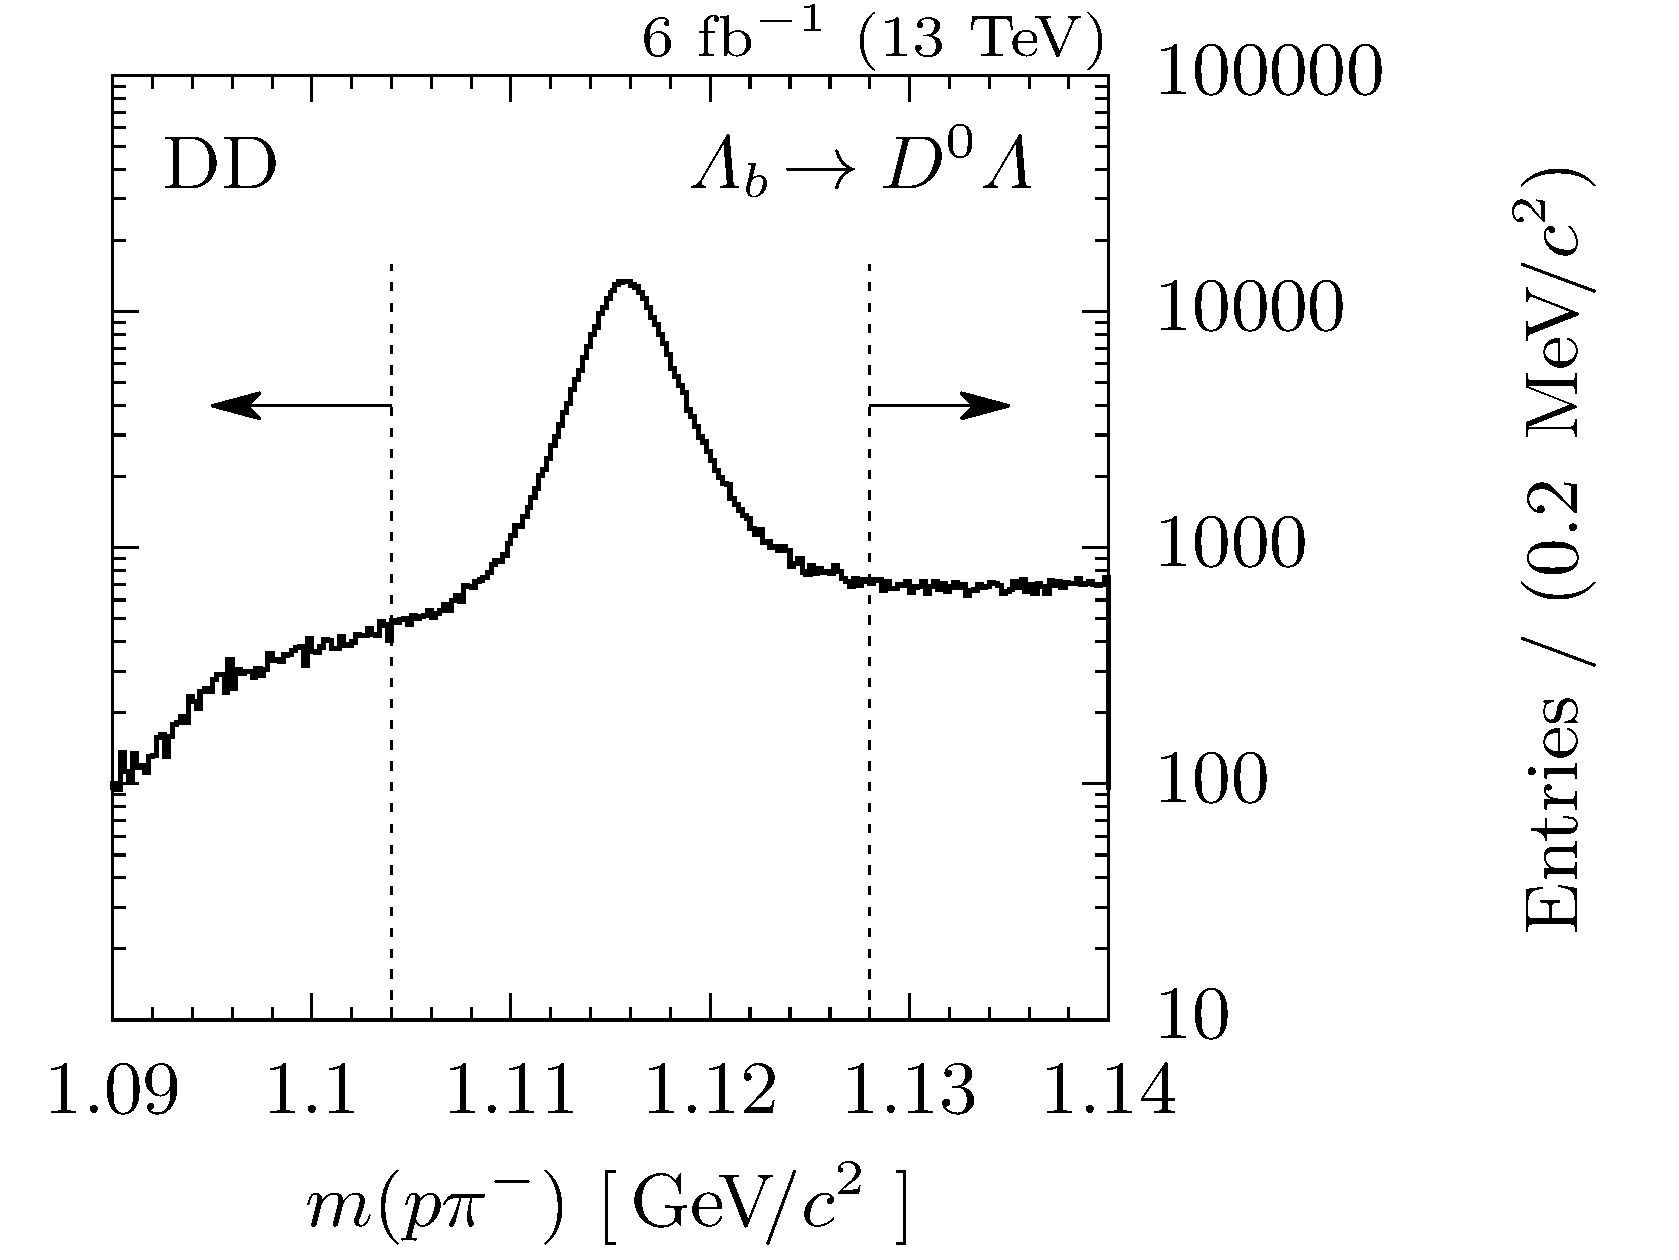
\includegraphics[scale=1.]{mva/hLzM_DD.png}
    \end{subfigure}
    \caption{Invariant masses of the \Dz candidates (top) and \Lz candidates (bottom), reconstructed from recorded data that are classified as \textit{signal} \decay{\Lb}{\Dz\Lz} decays by the final \gls{mva} classifier.}
    \label{fig:mva_hm}
\end{figure}

\begin{figure}[htbp]
    \centering
    \begin{subfigure}{.49\textwidth}
        \centering
        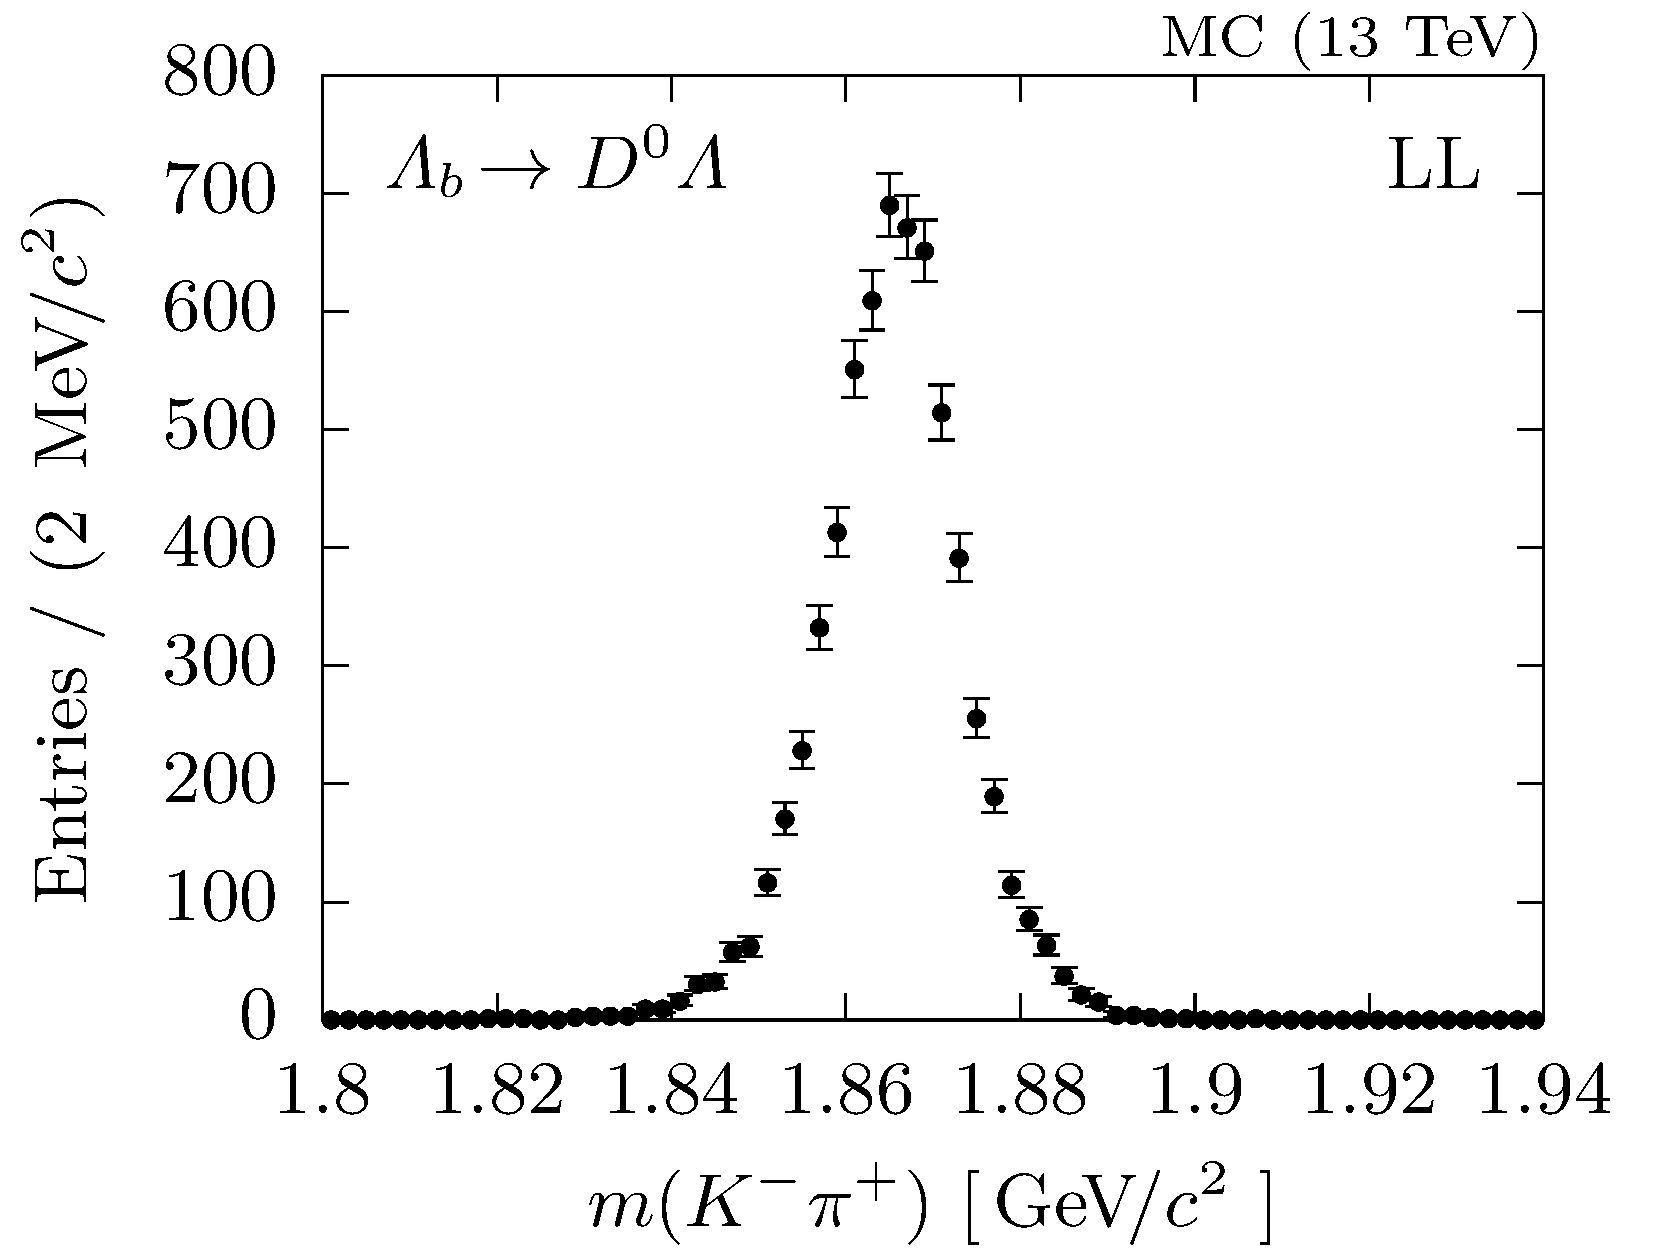
\includegraphics[scale=1.]{mva/hDzM_LL_MC.png}
    \end{subfigure}
    \begin{subfigure}{.49\textwidth}
        \centering
        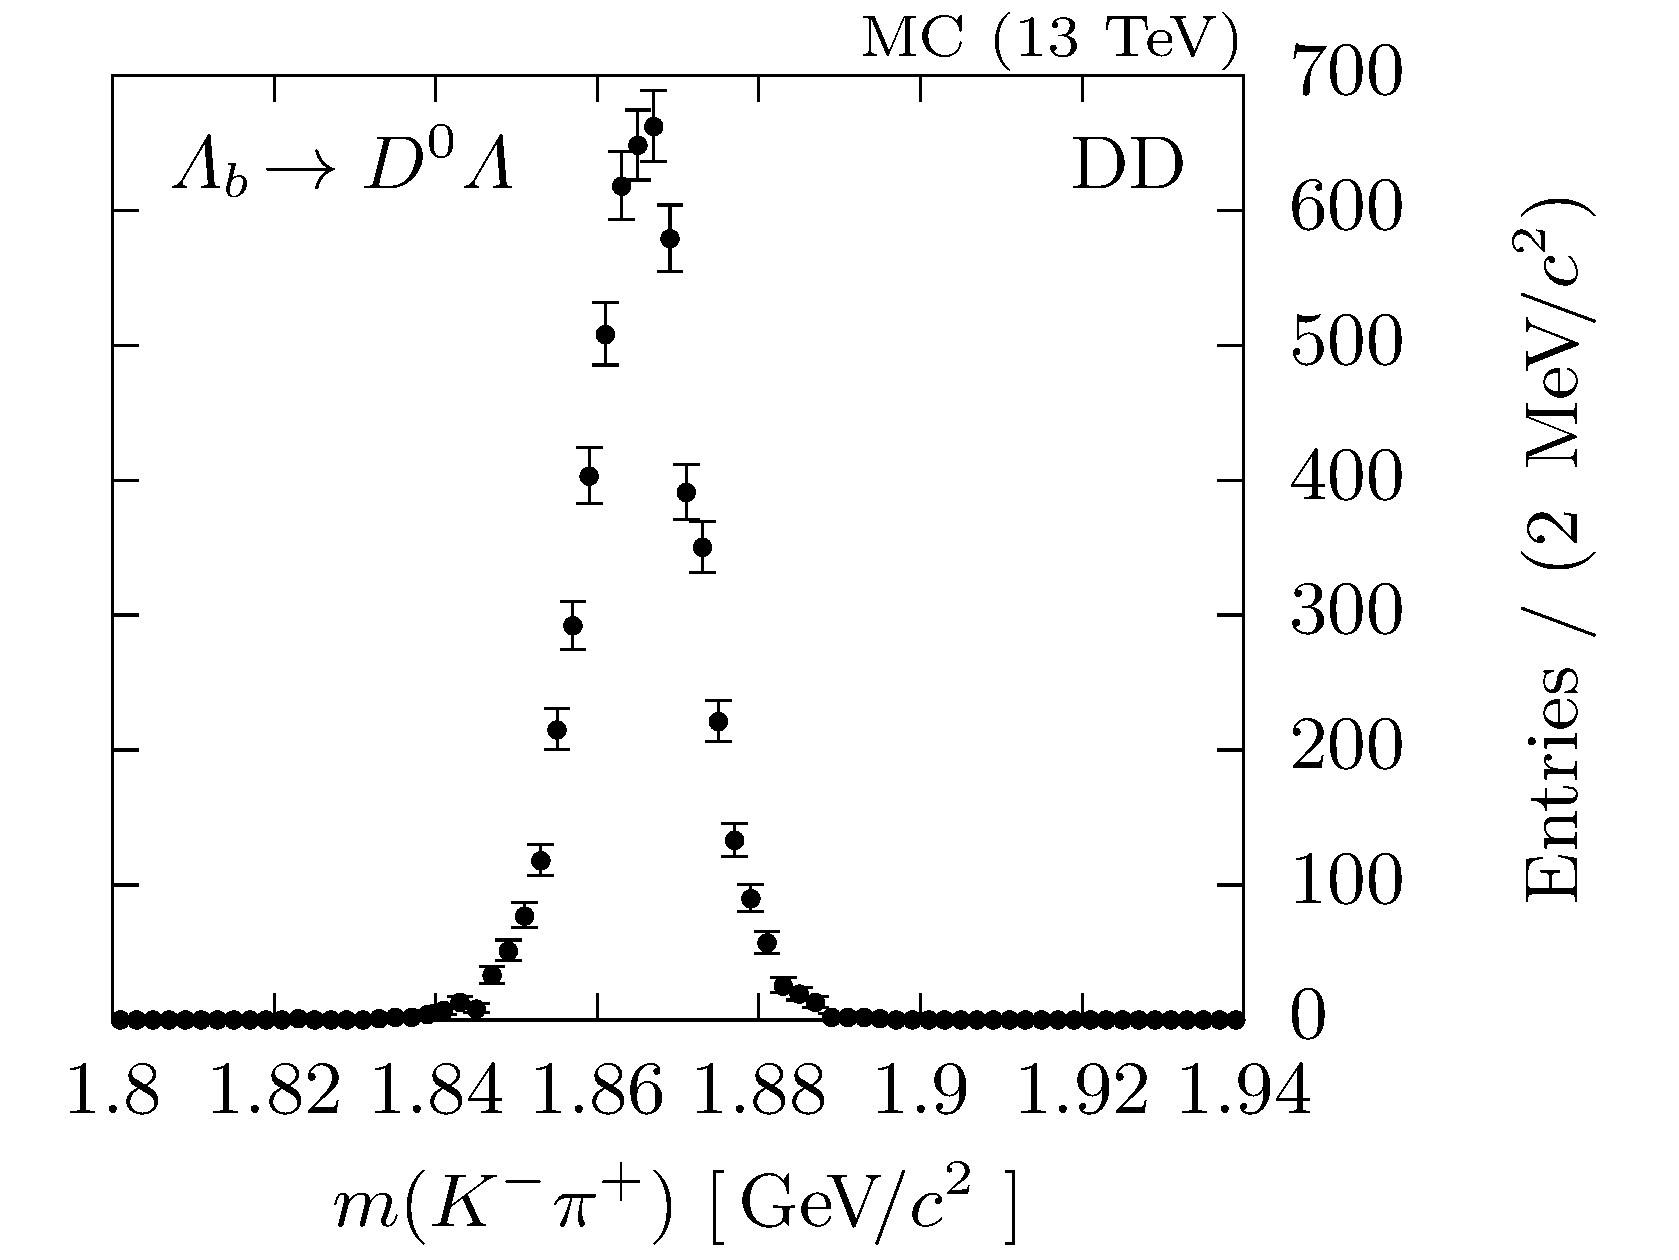
\includegraphics[scale=1.]{mva/hDzM_DD_MC.png}
    \end{subfigure}
    \par\bigskip 
    \begin{subfigure}{.49\textwidth}
        \centering
        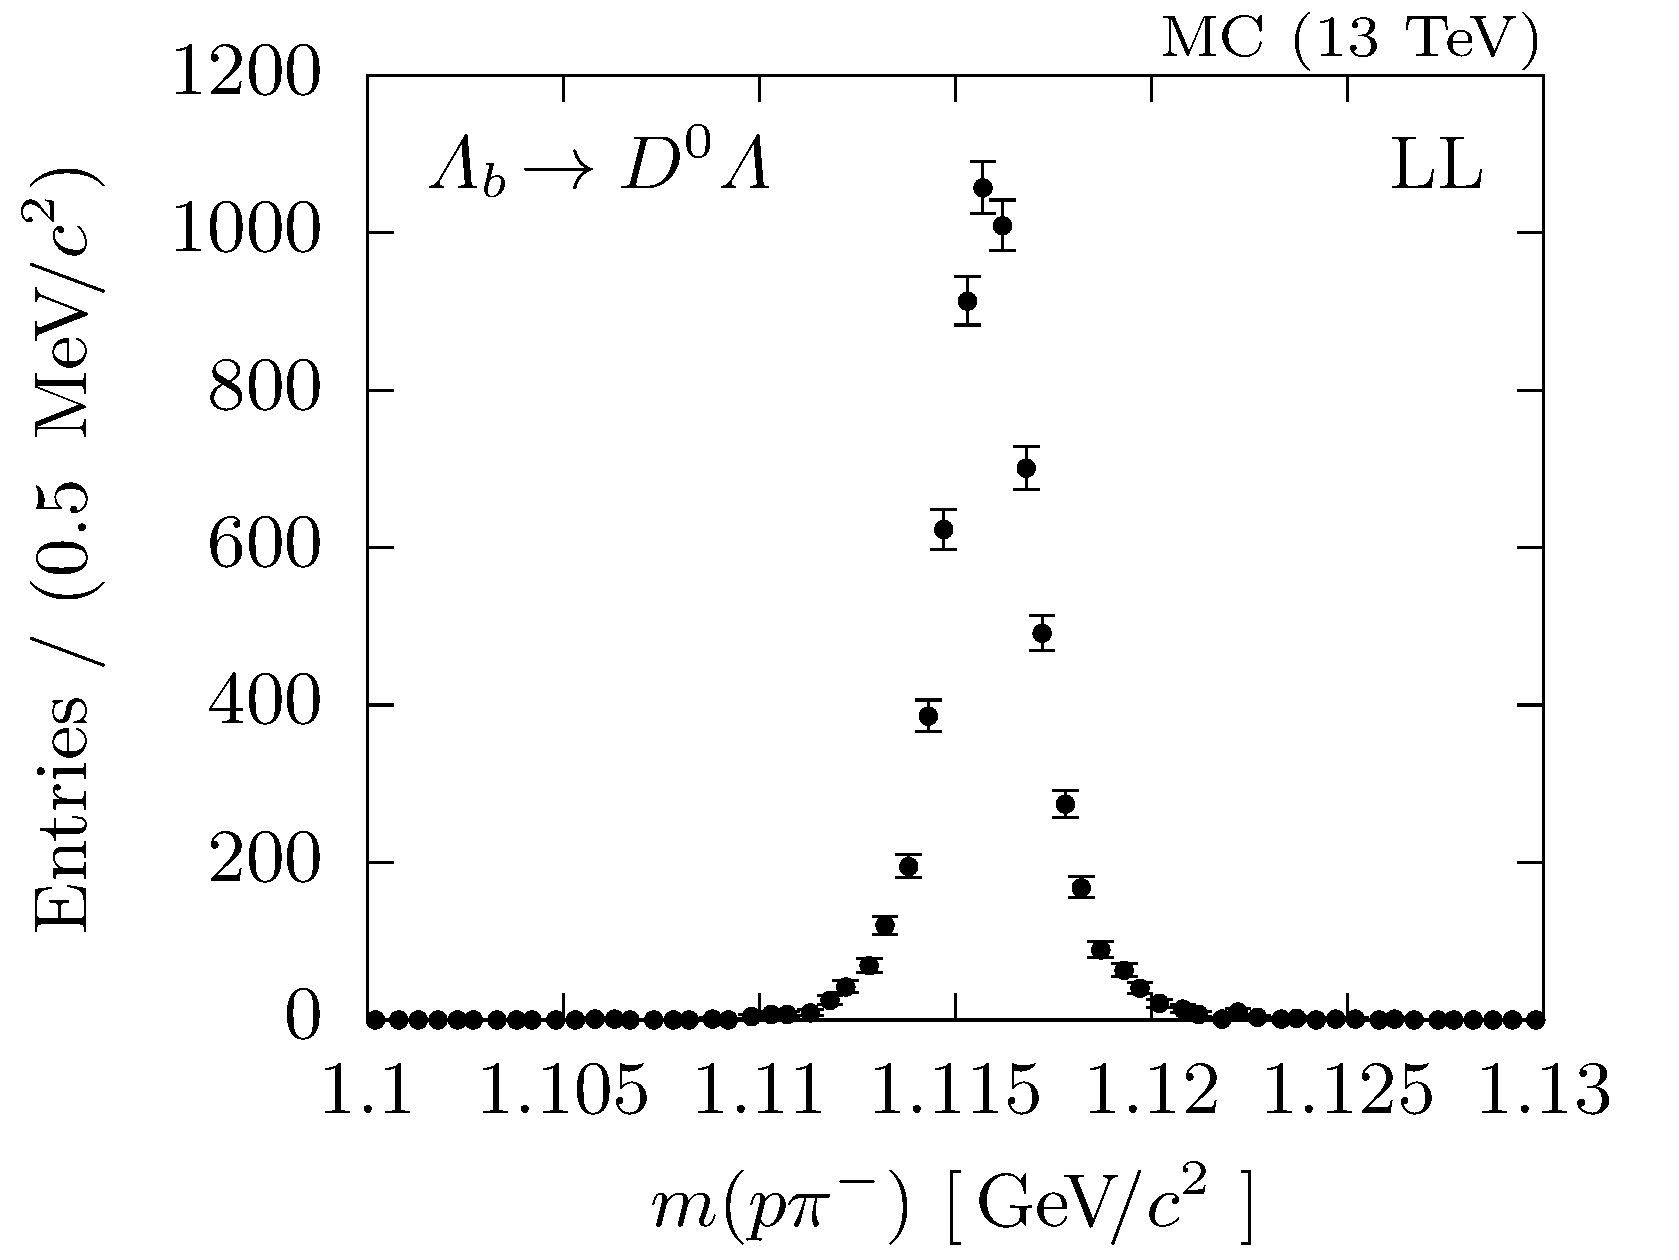
\includegraphics[scale=1.]{mva/hLzM_LL_MC.png}
    \end{subfigure}
    \begin{subfigure}{.49\textwidth}
        \centering
        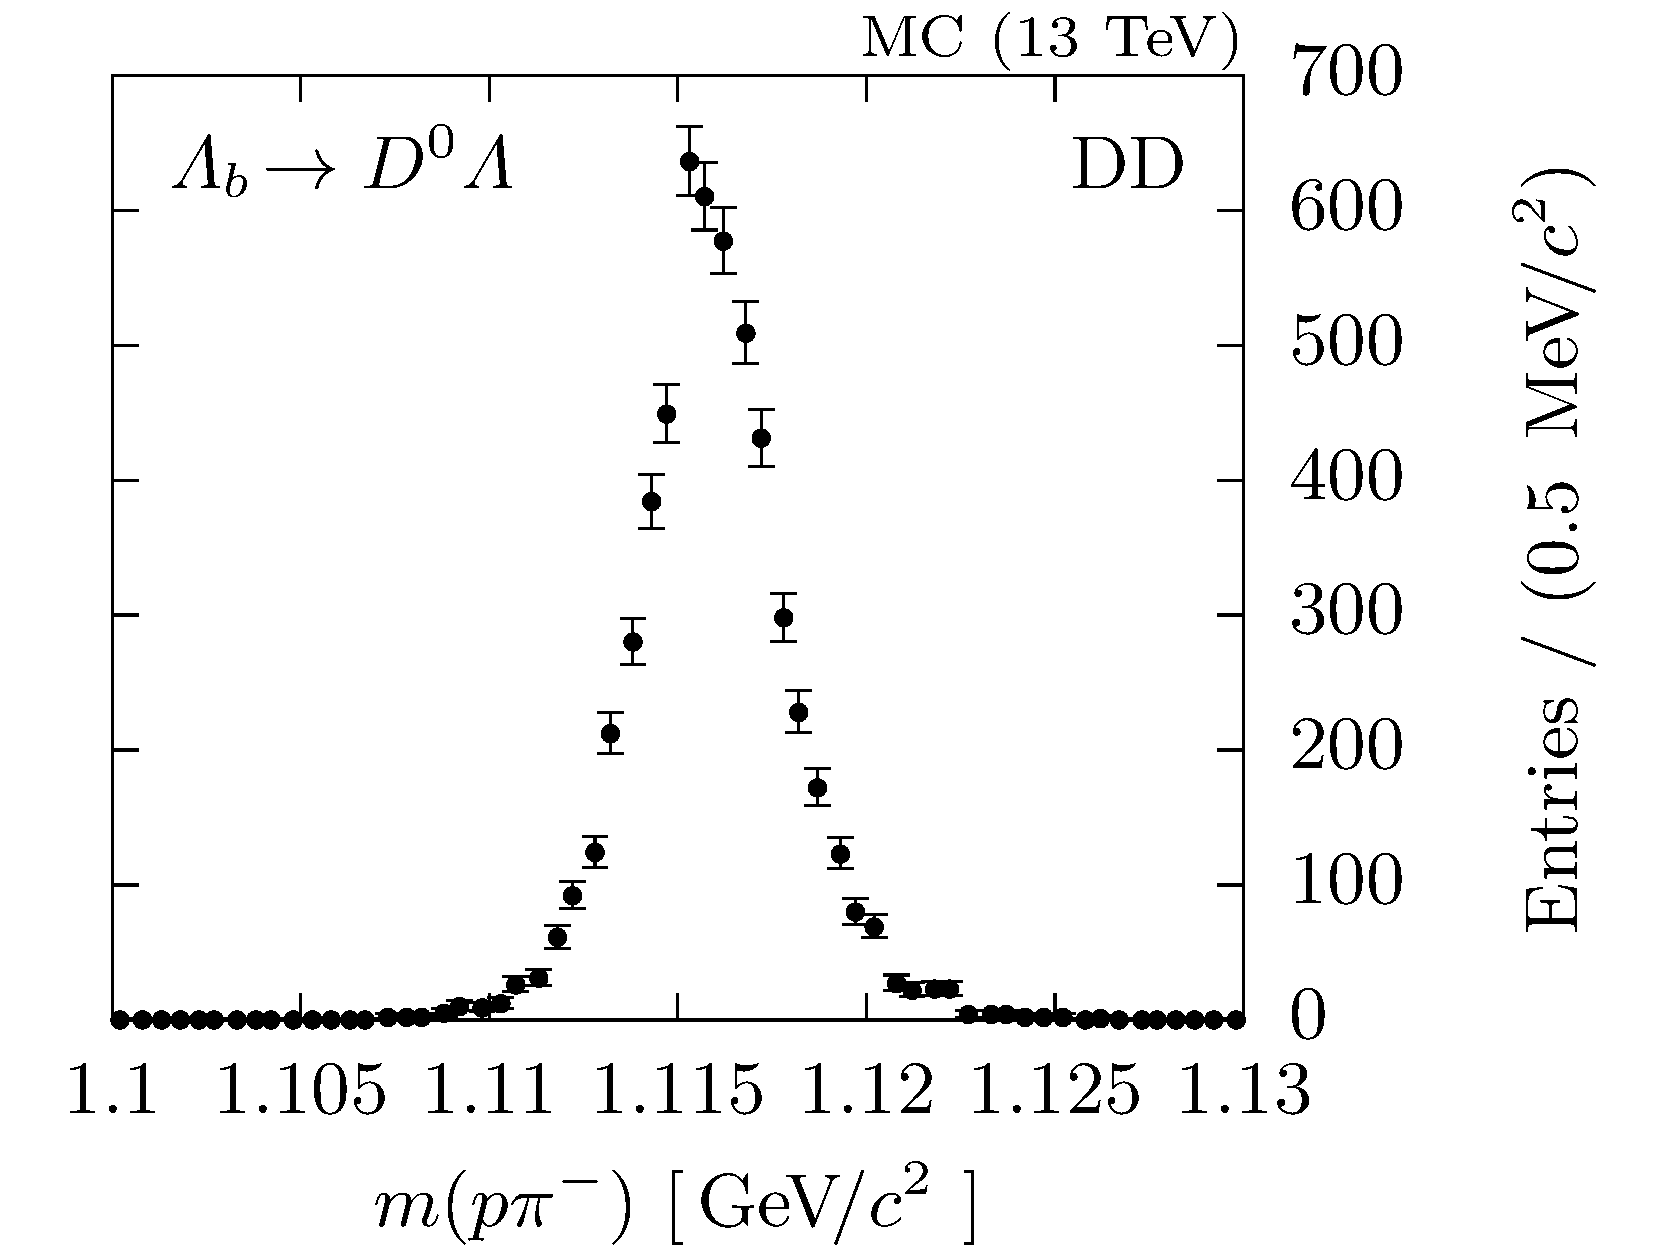
\includegraphics[scale=1.]{mva/hLzM_DD_MC.png}
    \end{subfigure}
    \par\bigskip 
    \begin{subfigure}{.49\textwidth}
        \centering
        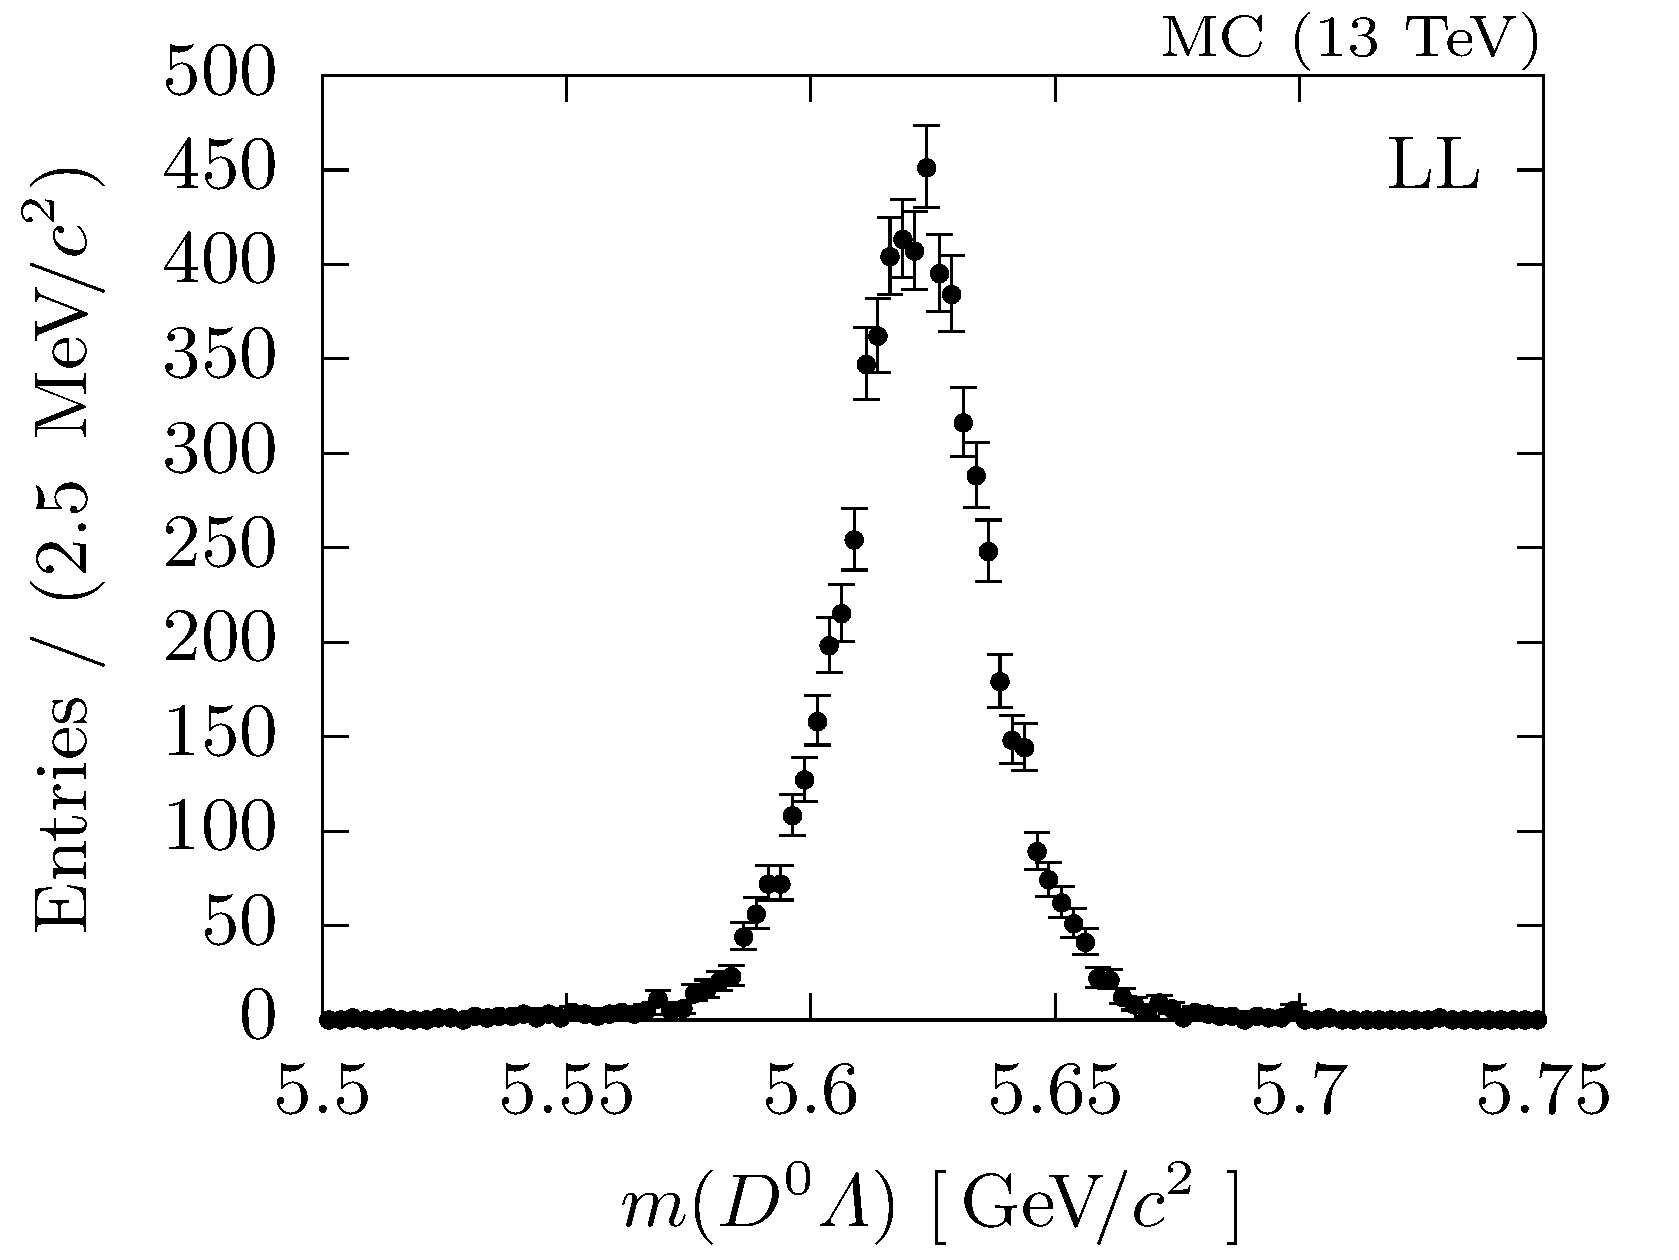
\includegraphics[scale=1.]{mva/hLbM_LL_MC.png}
    \end{subfigure}
    \begin{subfigure}{.49\textwidth}
        \centering
        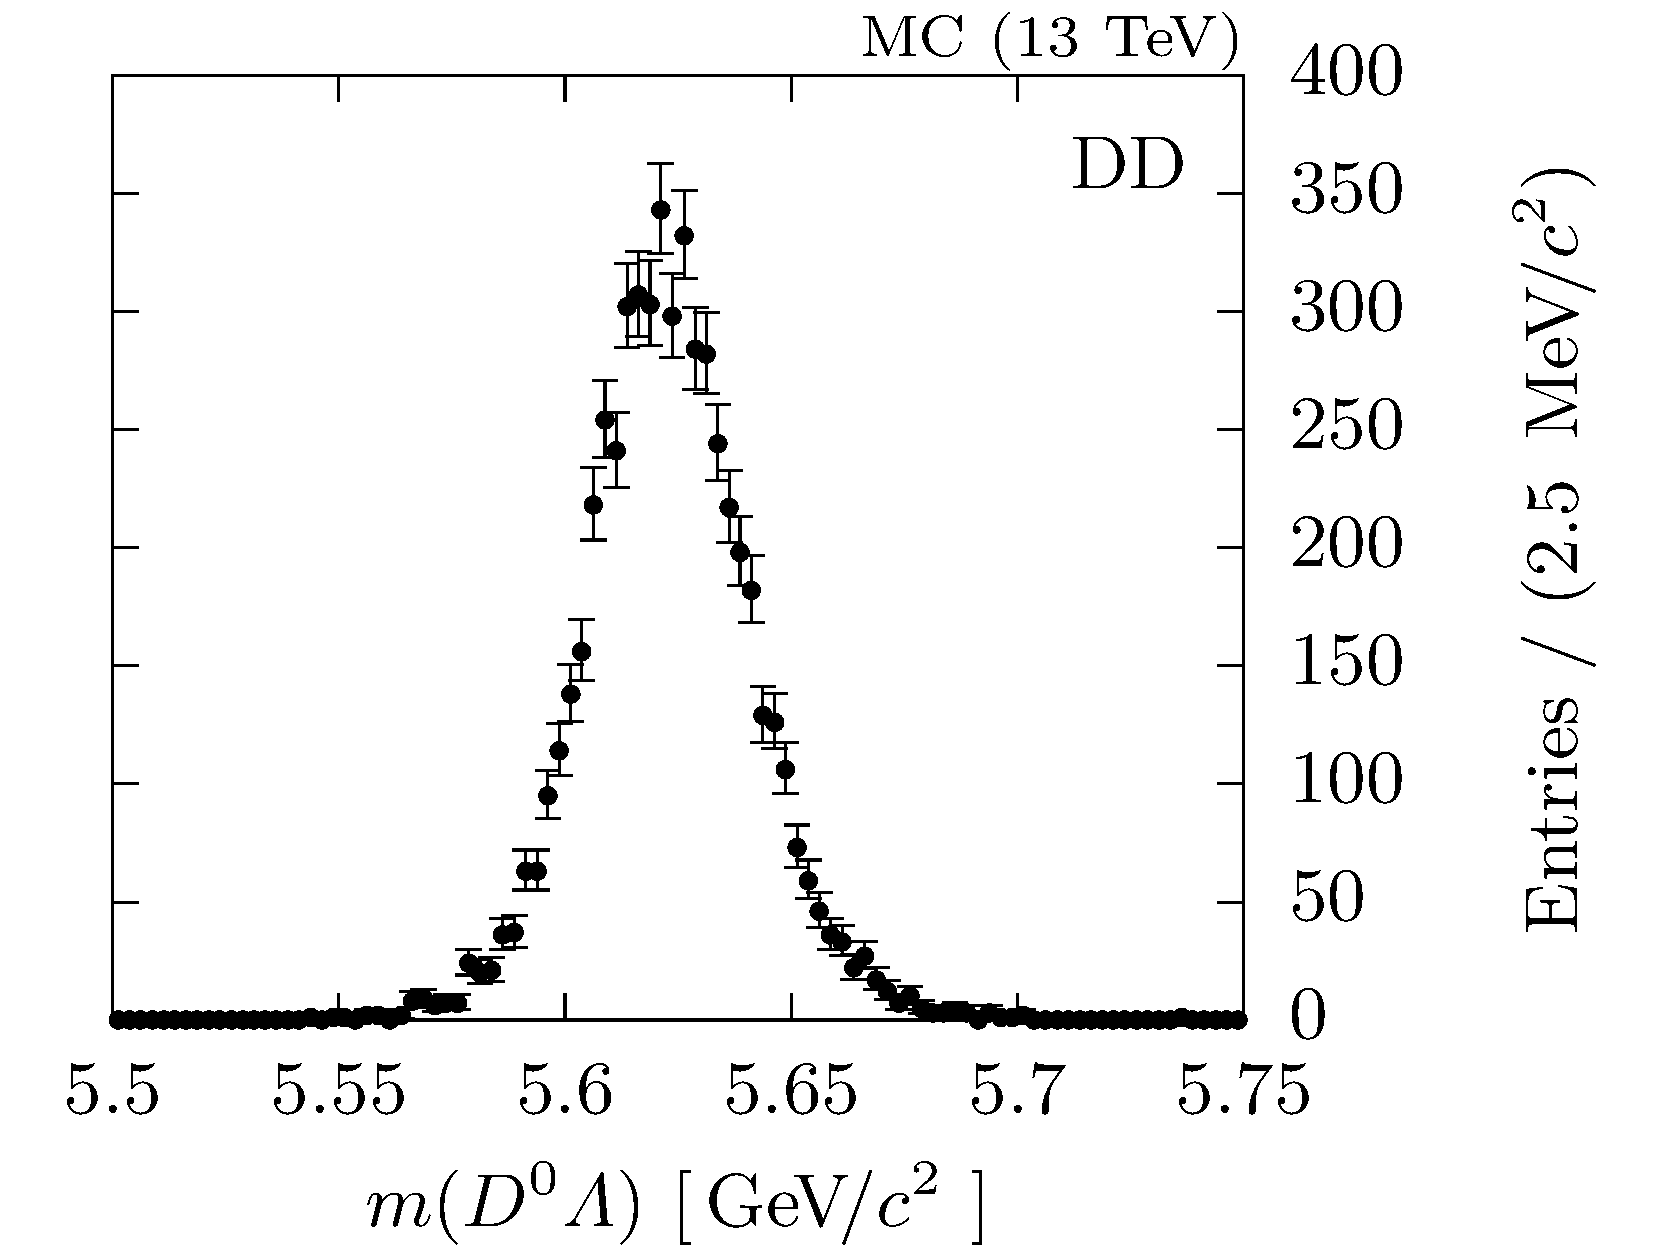
\includegraphics[scale=1.]{mva/hLbM_DD_MC.png}
    \end{subfigure}
    \caption{Invariant masses of \gls{mc} simulated \Dz, \Lz and \Lb candidates (top to bottom), \gls{truthmatched} as genuine \decay{\Lb}{\Dz\Lz} decays that are classified as \textit{signal} \decay{\Lb}{\Dz\Lz} decays by the final \gls{mva} classifier.}
    \label{fig:mva_hm_MC}
\end{figure}
